\documentclass[aspectratio=169,10pt]{beamer}
\usepackage{teaching_slides}
\usepackage{ragged2e}


\title{Conduct and Testing For Conduct}
\author{Chris Conlon}
\institute{Grad IO}
\date{Fall 2026}

\begin{document}

\frame{\titlepage}

\section{The problem}

\begin{frame}[plain]{Conduct Testing in Industrial Organization}
Foundational Empirical IO Question: How do we observe data on price and quantity and infer which model of firm behavior generated those outcomes?

\begin{itemize}
\item Early work: Porter (1983), Bresnahan (1982,1987)
\item Subsequent work defined the ``menu" approach: Nevo (1998, 2001), Villas-Boas (2007) 
\item Recent revival of ``internalization'' parameters: Miller and Weinberg (2017), Crawford, Lee, Whinston, and Yurukoglu (2017), Pakes (2017)
\item Parallel work by: Duarte, Magnolfi, S\o lvsten, Sullivan (QE 2024): which test is best (RV) and when instruments are too weak to test. Magnolfi, Quint, Sullivan, Waldfogel (2022): should we test or estimate?
\item Applications of our test: Starc and Wollmann (2022), Scuderi and Roussille (2025), others?
\item Today: the classic approaches, then the Backus--Conlon--Sinkinson test as it stands in the current draft (``BCS 2.0''), then what the cereal data taught us about what identifies conduct.
\end{itemize}
Is conduct testable? Berry and Haile (2014): yes.
\end{frame}


\begin{frame}{Conduct Testing in Industrial Organization}
\begin{itemize}
\item Absent additional restrictions, we cannot generally look at data on $(P,Q)$ and decide whether or not collusion is taking place.
\begin{itemize}
\item You say we started colluding at date $t$, I say we received a correlated shock to $mc$.
\end{itemize}
\item We can make progress in two ways: (1) parametric restrictions on marginal costs; (2) exclusion restrictions on supply.
\begin{itemize}
\item Most of the literature focuses on (1) by assuming something like: $\ln mc_{jt} = \textrm{x}_{jt} \gamma_1 + \textrm{w}_{jt} \gamma_2 + \omega_{jt}$.
\item In principle (2) is possible if we have instruments that shift demand for products but not supply. (These are much easier to come up with than ``supply shifters''). (This is the point Berry Haile 2014 make).
\end{itemize}
\end{itemize}
\end{frame}


\begin{frame}{A famous plot (Bresnahan 87)}
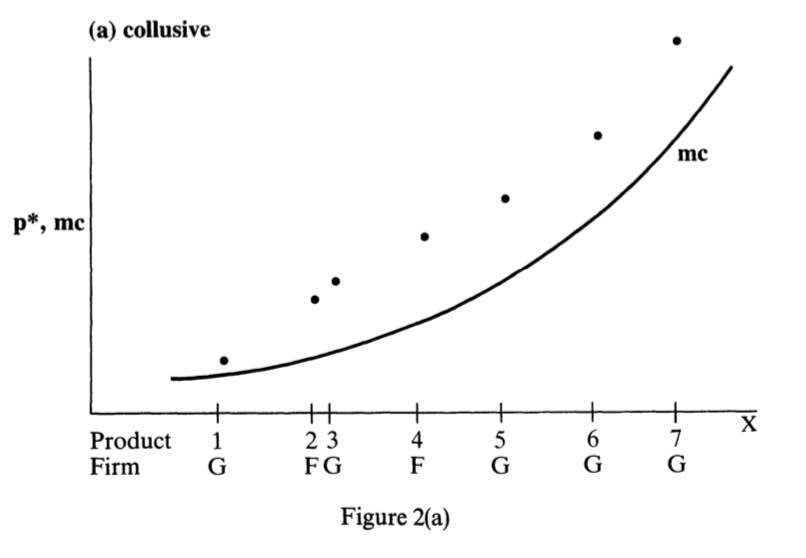
\includegraphics[width = 6.6cm]{./resources/bres_plot1.png}
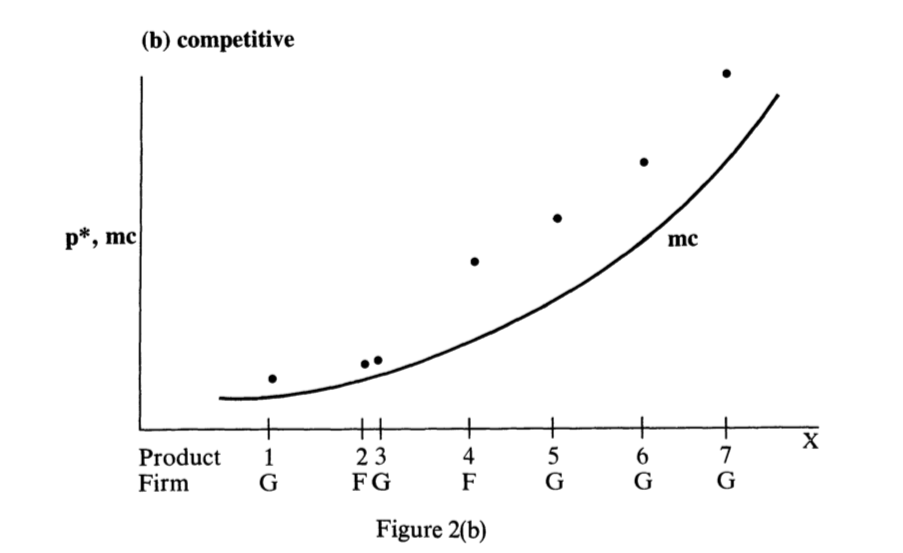
\includegraphics[width = 6.9cm]{./resources/bres_plot2.png}\\
Bresnahan (1980/1982) recognized this problem: we need ``rotations of demand''.
\end{frame}


\begin{frame}[plain]{Conduct Testing in Pictures (Berry Haile 2014)}
\begin{center}
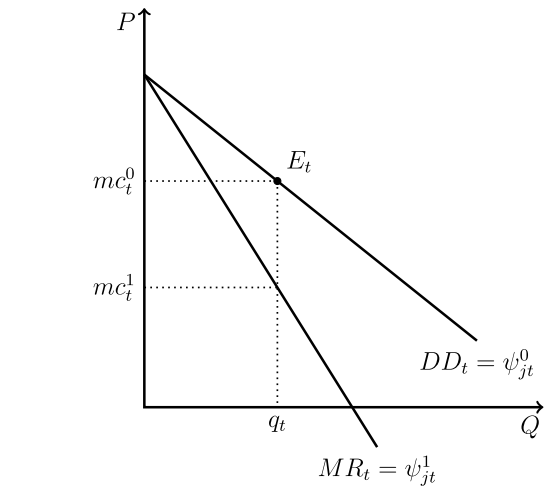
\includegraphics[width = 6.5cm]{resources/berryhaile1.png}
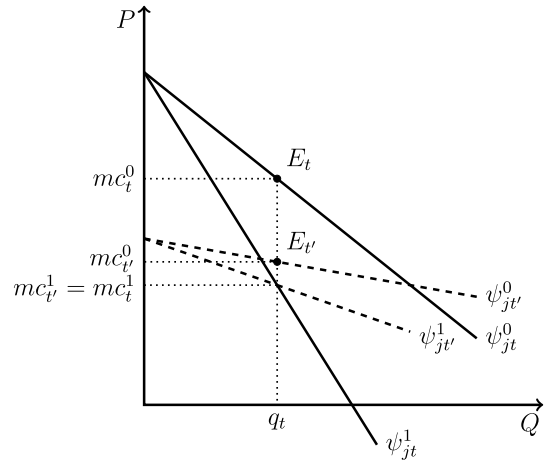
\includegraphics[width = 6.5cm]{resources/berryhaile2.png}
\end{center}
\small{Figure 2(ab) from Berry and Haile (2014), Example 1.}
\end{frame}


\begin{frame}{Setup: Notation and Utility}
We begin with a relatively standard BLP-style differentiated products setup.\\

\begin{itemize}
    \item Markets $t$
    \item Products $j$
    \item Data $\chi_t = \{(\textrm{x}_{jt},\textrm{v}_{jt},\textrm{w}_{jt})$ for all $j \in \calJ_t\}$.
    \item Market Shares $\symbf{s}_t = [s_{1t}, \ldots, s_{Jt}, s_{0t}]$.
    \item Prices $\symbf{p}_t = [p_{1t}, \ldots, p_{Jt}]$.
    \item Consumers $i$ with demographics $\textrm{y}_{it}$ (income, presence of kids, etc.)
\end{itemize}
\end{frame}


\begin{frame}
\frametitle{Testing Conduct: Multiproduct Bertrand Example}
\small
We generalize the $\mathcal{H}(\kappa)$ and derive multi-product Bertrand FOCs:
\begin{align*}
\arg \max_{p \in \calJ_f} \pi_f (\symbf{p}) &= \sum_{j \in \calJ_f} (p_j - c_j) \cdot q_j(\symbf{p}) +  \alert{\kappa_{fg} \sum_{j \in \calJ_g} (p_j - c_j) \cdot q_j(\symbf{p})} \\
\rightarrow 0&= q_j(\symbf{p}) + \sum_{k \in (\calJ_f,\calJ_g)} \alert{\kappa_{fg}}\cdot (p_k - c_k) \frac{\partial q_{k}}{\partial p_j}(\symbf{p}) 
\end{align*}
\begin{itemize}
\item Instead of $0$'s and $1$'s we now have $\kappa_{fg} \in [0,1]$ representing how much firm $f$ cares about the profits of $g$.
\begin{itemize}
\item If $f$ and $g$ merge (or fully coordinated) then $\kappa_{fg} =1$
\item Often in the real world firms cannot reach fully collusive profits and $\kappa_{fg} \in (0,1)$.
\item Evidence that $\kappa_{fg} > 0$ is not necessarily evidence of malfeasance, just a deviation from \alert{static Bertrand pricing} (e.g. Cournot, Dynamics, etc.)
\end{itemize}
\end{itemize}
\end{frame}


\begin{frame}{Testing Conduct: Multiproduct Bertrand Example}
\begin{itemize}
\item Recall the $\Delta$ matrix which we can write as $\Delta=\tilde{\Delta}\, \odot \mathcal{H}(\kappa)$, where $\odot$ is the element-wise or Hadamard product of two matrices. 
\begin{itemize}
\item $\tilde{\Delta}$ is the matrix of demand derivatives with $\Delta{(j,k)} = \frac{\partial q_j}{\partial p_k}$ for all elements.
\item $\mathcal{H}(\kappa)=\kappa_{fg}$ for products owned by $(f,g)$ where $\kappa_{ff}=1$ always.
\end{itemize}
\item Mergers are about changing $0$'s to $1$'s in the $\mathcal{H}(\kappa)$ matrix.
\item Matrix form of FOC: $q(\symbf{p}) = \Delta(\symbf{p},\kappa)\cdot(\symbf{p}-\symbf{mc})$
\item $\symbf{mc} =  \symbf{p} - \underbrace{\Delta(\symbf{p}, \theta_2, \kappa)^{-1} \symbf{\sigma}(\symbf{p})}_{\eta(\symbf{p},\symbf{s},\theta_2,\kappa)}$
where $\eta_{jt}$ is the markup.
\end{itemize}
\end{frame}


\begin{frame}
\frametitle{Reasons for Deviations from Multiproduct Bertrand}
\small
\begin{description}
\item[Biased estimates of own and cross price derivatives:] For anything to work, you have correct estimates of $\tilde{\Delta}$. My prior is most papers \alert{underestimate} diversion ratios for close substitutes.
\item[Vertical Relationships:] Who sets supermarket prices? Just the retailer? Just the manufacturer? Some combination of both? Retailers tend to \alert{soften} downstream price competition.
\item[Faulty Timing Assumptions:] Bertrand is a simultaneous move pricing game. Lots of alternatives (Stackelberg leader-follower, Edgeworth cycles, etc.).
\item[Dynamics and Dynamic Pricing:] Forward looking firms or consumers might not set static Nash prices. [e.g. Temporary Sales, Switching Costs, Network Effects, etc.]
\item[Unmodeled Supergame:] Maybe firms are legally tacitly colluding, higher prices might be about what firms believe will happen in a price war.
\end{description}
\end{frame}


\begin{frame}{Simultaneous Problem}
Assume additivity, and write in terms of structural errors:
\begin{align*}
\delta_{jt}(\symbf{s}_t,\alert{\textrm{y}_t}, \widetilde{\theta}_2) + \alpha p_{jt} &= h_d(\textrm{x}_{jt}, \, \alert{\textrm{v}_{jt}},\theta_1)  + \xi_{jt} \\
 f \left( p_{jt} - \eta_{jt}(\symbf{p},\symbf{s},\theta_2,\kappa) \right) &= h_s(\textrm{x}_{jt}, \alert{\textrm{w}_{jt}},\theta_3) + \omega_{jt}
\end{align*}
\vspace{-.4cm}
\begin{itemize}
 \item To simplify slides we let $f(x)=x$ (often $f(x) =\log(x))$ but we can put that in $h_s(\cdot)$.
\item $h(\cdot)$ are often just linear relationships like: $\theta_1 [\textrm{x}_{jt}, \textrm{v}_{jt}]$.
\item Endogeneity Problem: $p_{jt}$ and $\eta_{jt}$ are functions of $(\symbf{\xi},\symbf{\omega})$.
\item $(\theta_2, \kappa)$ parameters that determine markups
\end{itemize}
\end{frame}


\begin{frame}{Two Ways In (Recap of the BLP Lecture)}
\begin{enumerate}
\item \textbf{Demand first.} Estimate $\theta_2$ from demand alone with $\E[\xi_{jt} \mid \textrm{x}_t, \textrm{v}_t, \textrm{w}_t] = 0$; recover $\widehat{\symbf{mc}} = \symbf{p} - \symbf{\eta}(\symbf{p}, \symbf{s}, \widehat{\theta}_2, \kappa)$ for \alert{any} $\kappa$.
\item \textbf{Jointly.} Stack the supply moments $\E[\omega_{jt} \mid \textrm{x}_t, \textrm{w}_t, \textrm{v}_t]=0$ with demand; the supply side sharpens $\alpha$ (BLP 1995) but imports whatever conduct you assumed.
\end{enumerate}
The problem with either: given $[\symbf{q}, \symbf{p}, \widetilde{\Delta}, \calH(\kappa)]$ there is \alert{always} a vector $\symbf{mc}$ that rationalizes the data ($J$ equations, $J$ unknowns). Nonparametrically $\kappa$ is not identified without more.
\begin{itemize}
\item Restriction 1: a model of marginal cost, $f(p_{jt} - \eta_{jt}(\kappa)) = h_s(\textrm{x}_{jt}, \textrm{w}_{jt}; \theta_3) + \omega_{jt}$, so that ``$mc < 0$'' or ``$mc$ jumps around'' become evidence.
\item Restriction 2: \alert{exclusion}. Something that moves markups but not costs, $\E[\omega_{jt} \mid z_{jt}] = 0$ (Berry Haile 2014: demand rotators $\textrm{v}_t$, rivals' characteristics).
\item Everything that follows is a way of turning those two restrictions into a test. The second one does all the real work.
\end{itemize}
\end{frame}


\section{Classic approaches}

\begin{frame}{Estimation vs. Menus}
There are 2.5 ways to think about conduct:
\begin{enumerate}
\item Using moment conditions to estimate $\widehat{\kappa}$ or $\mathcal{H}(\kappa)$ directly. (Wald)
\begin{itemize}
\item Often with a small number of parameters (ie: $\kappa_{fg}=0$ except for firms I know are in a cartel).
\item Can be challenging to tell similar values of $\kappa_{fg}$ apart (under-powered).
\end{itemize}
\item ``Menu Approach'' / (LR)
\begin{itemize}
\item  Nevo (Economics Letters 1998)
\item Bresnahan (1987)
\item Compare some goodness-of-fit critieria across assumed values of $\kappa$ (Bertrand vs. Collusion)
  \end{itemize}
\item Rejecting (or failing to reject) a single model.
\begin{itemize}
  \item ``We can reject monopoly pricing...''
\end{itemize}
  \end{enumerate}
\end{frame}


\begin{frame}{Testing a single model of $\kappa$}
Put the $\eta_{jt}$ on the RHS and test whether $\lambda=1$:
\begin{align*}
 p_{jt} = h_s(\textrm{x}_{jt}, \alert{\textrm{w}_{jt}},\theta_3) + \lambda \cdot \eta_{jt}\left(\symbf{p},\symbf{s},\theta_2,\kappa \right)+  \omega_{jt} \text{ with }
 \E[\omega_{jt} | \textrm{x}_{t},\textrm{w}_{t},z_{t}]=0
\end{align*}
\vspace{-0.25cm}
\begin{itemize}
\item We are basically running 2SLS with IV for the endogenous $\eta_{jt}$
\item ``Informal'' test of Villas Boas (2007): $\E[\omega_{jt} | \textrm{x}_{jt},\alert{\textrm{w}_{jt}},\alert{\eta_{jt}}]=0$.
\begin{itemize}
\item Considers different forms of $f(\cdot)$: linear, exponential, logarithmic.
\item WP discusses this more than Restud version.
  \end{itemize}
\item Pakes (2017) uses Wollman (2018) data and BLP IV $\E[\omega_{jt} \mid \textrm{x}_{jt},\textrm{w}_{jt},f(\textrm{x}_{-j})]=0$.
\item $\lambda \neq 0$ is hard to interpret.
\end{itemize}
\end{frame}


\begin{frame}{Pakes (2018)/Wollman (2017) Regressions: Heavy Trucks}
\begin{center}
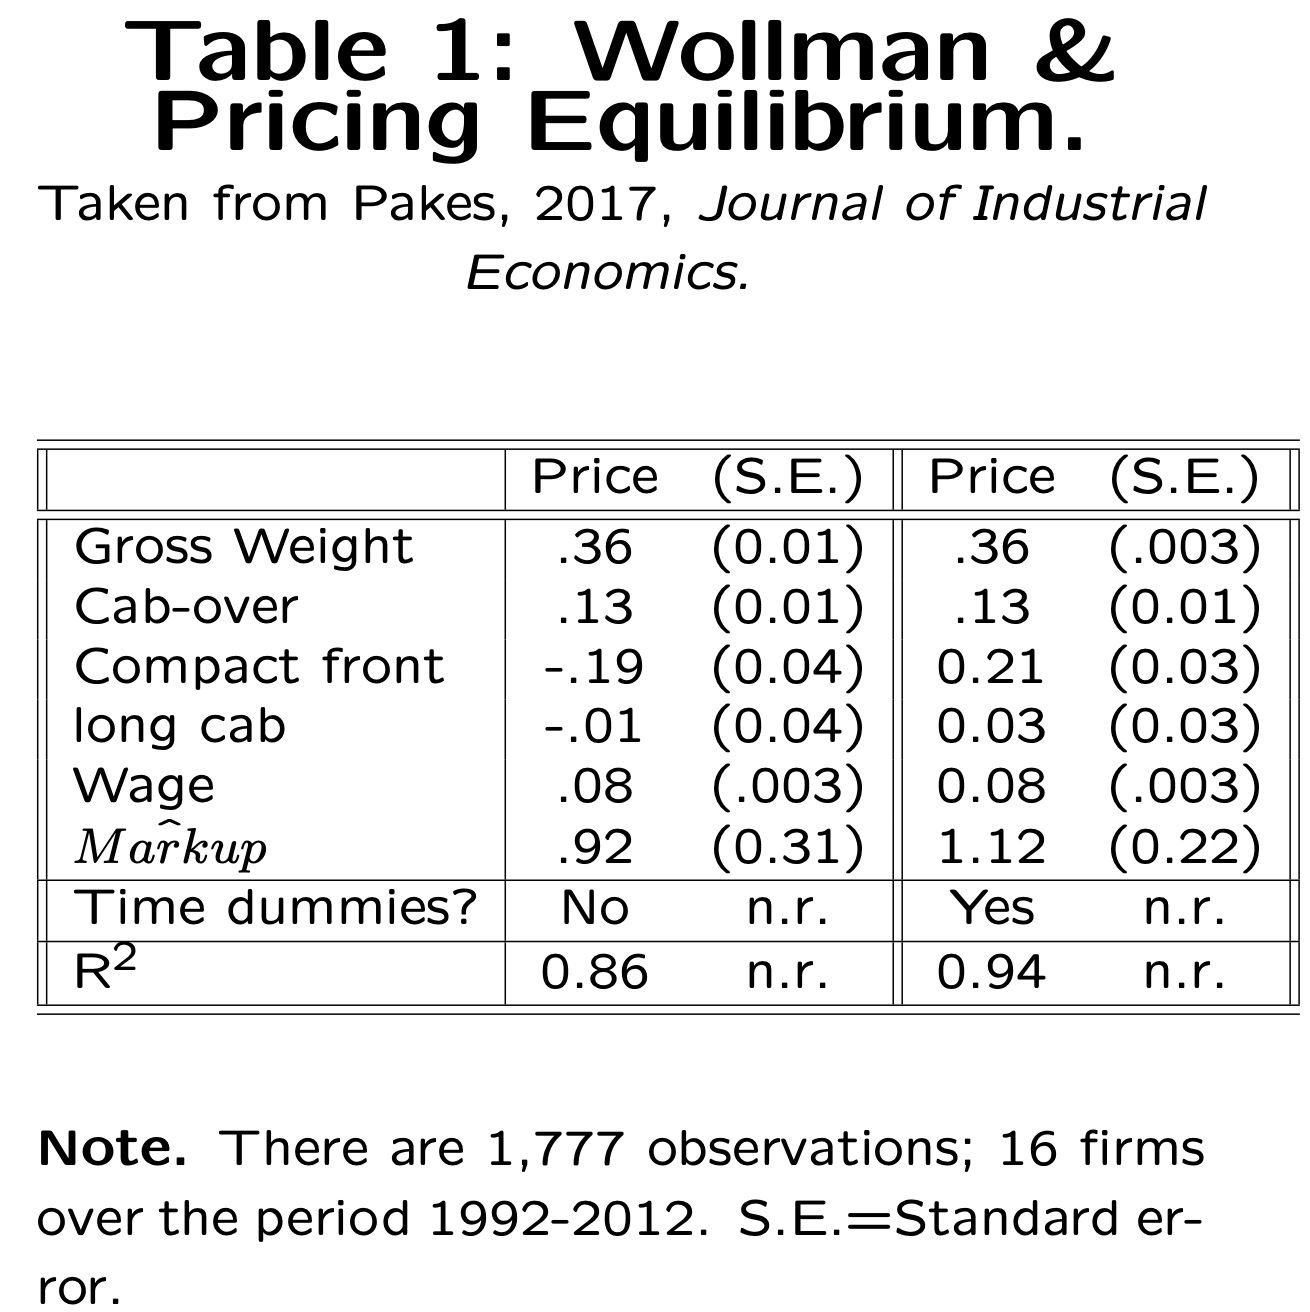
\includegraphics[height=0.9\textheight]{./resources/wollman_regression.png}
\end{center}
\end{frame}


\begin{frame}{Single Model Regressions}
These are somewhat reassuring:
\begin{itemize}
\item $\lambda\approx 1$ for multiproduct-oligopoly
\item Fit is pretty good $R^2 > 0.8$ and $R^2 > 0.5$ for within vehicle regressions (not shown).
\item As a behavioral model, multiproduct demand estimation seems successful.
\item But, do we know that an alternative $\mathcal{H}(\kappa)$ would have a $\lambda \neq 1$ or a lower $R^2$, and if so how low before we can ``reject'' the model?
\end{itemize}
\end{frame}


\begin{frame}{Goodness of Fit Tests}
Another idea (Bonnet and Dubois, Rand 2010) runs the following regression:
\begin{align*}
\log \left( p_{jt} - \eta_{jt}(\symbf{p},\symbf{s},\widehat{\theta}_2,\kappa) \right) &= h_s(\textrm{x}_{jt}, \alert{\textrm{w}_{jt}},\theta_3) + \omega_{jt}
\end{align*}
\begin{itemize}
\item Run a regression for each $\kappa$ and obtain $Q(\kappa)=\sum_{jt} \widehat{\omega}_{jt}^2$
\item Employ the \alert{non nested test} of Rivers and Vuong (2002). Why?
\item Working out the distribution of $Q(\kappa_1) - Q(\kappa_2)=T(\kappa_1,\kappa_2)$ is the hard part.
\item Also this is OLS (or NLLS) and there are no instruments or \alert{exclusion restrictions} for the supply side. Presumably we could add some and do GMM? (I think this is the ``formal'' test of Villas Boas (ReStud 2007)).
\end{itemize}
\end{frame}


\begin{frame}{Villas Boas (2007)}

\begin{columns}
\begin{column}{0.5\textwidth}
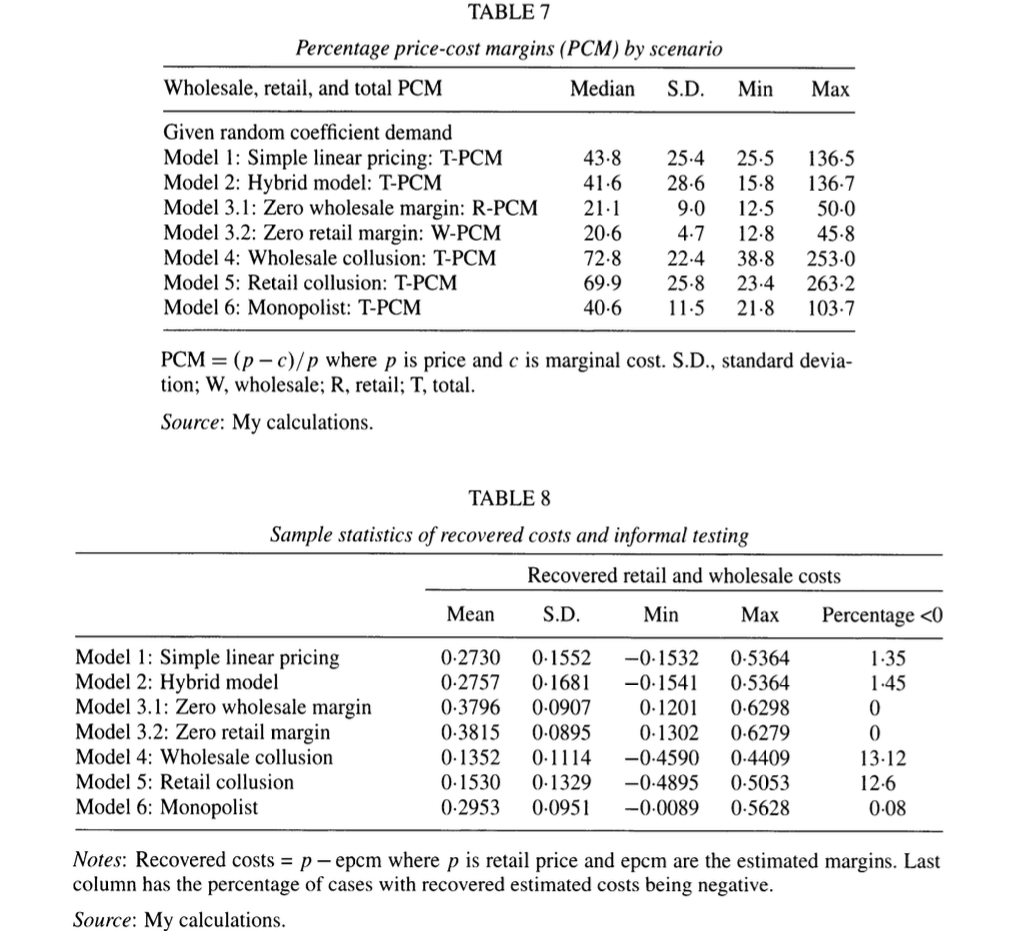
\includegraphics[height=0.9\textheight]{resources/villas_boas_table8.png}
\end{column}
\begin{column}{0.5\textwidth}
\begin{itemize}
\item Try out different models of price setting behavior, compute $\eta$ markups.
\item Unsurprisingly models with higher markups also have more costs $MC < 0$.
\item Is this evidence of incorrect conduct assumption or inelastic demand?
\end{itemize}
\end{column}
\end{columns}
\end{frame}


\begin{frame}{Villas Boas (2007)}
\begin{columns}
\begin{column}{0.6\textwidth}
\begin{center}
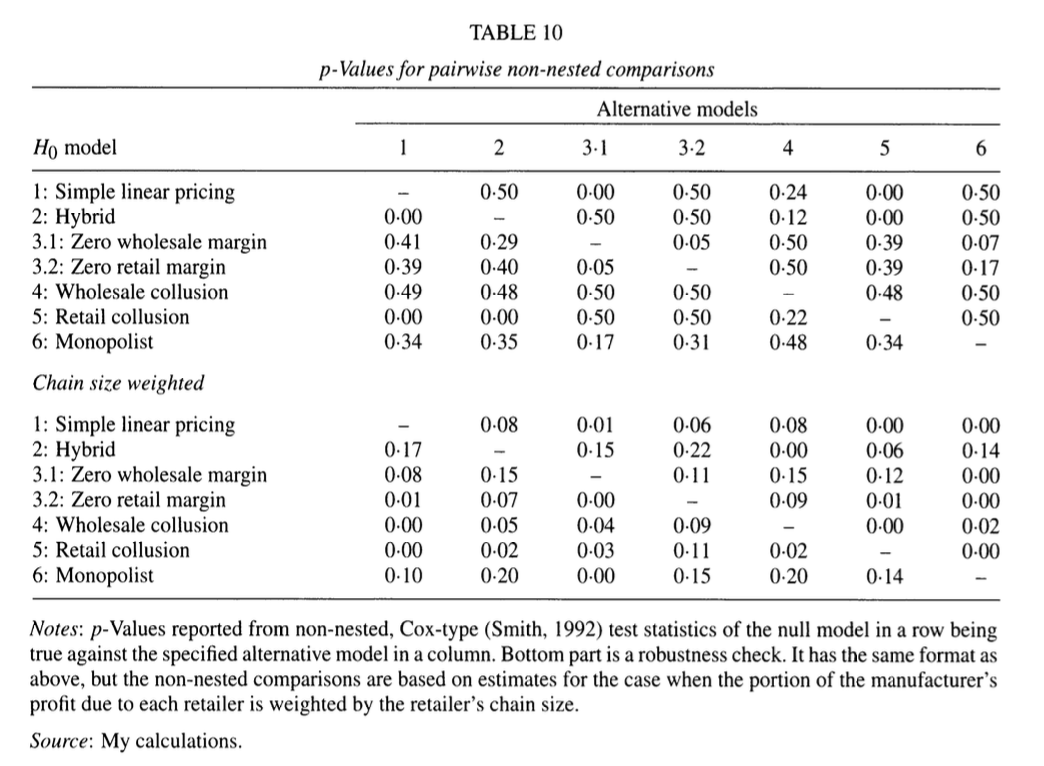
\includegraphics[height=0.9\textheight]{resources/villas_boas_table10.png}
\end{center}
\end{column}
\begin{column}{0.4\textwidth}
\begin{itemize}
\item Cox test has pairwise rejection problem (4) rejects (5) and (5) rejects (4).
\item Likewise for 3.1 and 3.2 in top panel.
\end{itemize}
\end{column}
\end{columns}


\end{frame}


\begin{frame}{Recap}
\small
So far three approaches to exploit $ \E[\omega_{jt} | \textrm{x}_{t}, \textrm{w}_{t}, z_{t}]=0$
\begin{enumerate}
\item Put the markup on RHS and instrument for it to test $\lambda=1$ (Wald)
\begin{align*}
 p_{jt} &= h_s(\textrm{x}_{jt}, \alert{\textrm{w}_{jt}},\theta_3) + \lambda \cdot \eta_{jt}\left(\symbf{p},\symbf{s},\widehat{\theta_2},\kappa \right)+  \omega_{jt}
\end{align*}
\item Put the markup on LHS assuming $\lambda=1$ and test goodness of fit of supply equation (Anderson Rubin)
\begin{align*}
 p_{jt} -\eta_{jt}\left(\symbf{p},\symbf{s},\widehat{\theta_2},\kappa \right)&= h_s(\textrm{x}_{jt}, \alert{\textrm{w}_{jt}},\theta_3) +  \omega_{jt}
\end{align*}
\item Estimate supply and demand simultaneously $[\theta_1,\theta_2,\theta_3]$ and compare goodness of fit for different $\kappa$. (Likelihood Ratio)
\end{enumerate}

\end{frame}


\begin{frame}{Which Test? Duarte, Magnolfi, S\o lvsten, Sullivan (QE 2024)}
\small
Take the supply equation seriously as a \alert{moment condition} and ask which classical test to run on a menu of markups $\{\eta^m\}$:
\begin{itemize}
\item \textbf{Specification tests} of one model at a time (Wald on $\lambda=1$, Anderson--Rubin / GMM-$J$ on $\E[\omega^m z]=0$, Cox): with enough data \alert{every} model is rejected, because no conduct model is exactly right. Villas-Boas's Cox test rejecting in both directions is the symptom.
\item \textbf{Model selection} (Rivers--Vuong 2002): compare two models' GMM criteria, $Q_W(\eta^{m_1}) - Q_W(\eta^{m_2})$, under the null that they are \alert{equally} misspecified. Only RV behaves sensibly when both models are wrong, which is always.
\item The catch: RV is \alert{degenerate} when the two models are indistinguishable through the instruments. DMSS define \alert{weak instruments for testing}, extend Stock--Yogo to model selection, and give an effective-$F$ diagnostic with critical values for worst-case size and best-case power (\texttt{pyRVtest}).
\item Their criterion is a finite-dimensional 2SLS quadratic form, $\bar{\symbf{m}}_m' (z'z)^{-1} \bar{\symbf{m}}_m$ with $\bar{\symbf{m}}_m = \frac{1}{n}\sum_i z_i \omega^m_i$ (a $K$-vector of unconditional moments). Keep that in mind: the two BCS criteria below are a \alert{single optimal direction} and the \alert{full conditional-moment norm}, and the DMSS object is the finite-$K$ thing in between.
\end{itemize}
\end{frame}


\section{The reframe: model selection under misspecification}

\begin{frame}{What Is the Null? Ranking Misspecified Models}
\small
Each conduct $m$ implies markups $\eta^m_{jt}$, hence an implied cost and a cost residual:
\begin{align*}
c^m_{jt} = p_{jt} - \eta^m_{jt} = h_s(\textrm{x}_{jt}, \textrm{w}_{jt}) + \omega^m_{jt}, \qquad
\mu_m(z) \equiv \E[\omega^m_{jt} \mid z_{jt}], \qquad
Q(\eta^m) \equiv \| \mu_m \|^2 = \E[\mu_m(z)^2] \geq 0 .
\end{align*}
\begin{itemize}
\item Correct conduct: $\mu_m \equiv 0$ and $Q(\eta^m) = 0$. On real data \alert{every} $Q(\eta^m) > 0$: no model on the menu satisfies the restriction exactly.
\item So the honest hypothesis is not ``Bertrand is true'' but Vuong (1989) / Rivers--Vuong (2002) / Chen--Hong--Shum (2007):
\begin{align*}
H_0: Q(\eta^{m_1}) = Q(\eta^{m_2}) \quad (\text{equally wrong}) \qquad \text{vs.} \qquad H_A: \text{one is closer to the moment condition.}
\end{align*}
\item A ``test of conduct'' is therefore a \alert{ranking}: which markups are closest to $\E[\omega \mid z] = 0$. ``Model $m$ is in the model confidence set'' means it is the hardest to beat, not that it is correct.
\item The cost function $h_s$ is a nuisance; it is the \alert{pseudo-true} cost function under each (possibly wrong) conduct, well defined because the criterion is shared across models.
\end{itemize}
\end{frame}


\begin{frame}{Degeneracy: When Two Wrong Models Are the Same Wrong Model}
\begin{itemize}
\item The RV statistic is $\sqrt{n}\,(\widehat{Q}_1 - \widehat{Q}_2)/\widehat{\sigma}$. Its denominator is the variance of the \alert{difference} of the two models' moments, and it can be zero under the null.
\item That happens when the two conducts induce the \alert{same conditional moment}, $\mu_{m_1}(z) \equiv \mu_{m_2}(z)$: observational equivalence (Chen--Hong--Shum's $H_E$). No instrument can rank them; the normal approximation is meaningless; $\widehat{\sigma} \rightarrow 0$ and the $t$-statistic is $0/0$.
\item Three roads lead there:
\begin{enumerate}
\item \textbf{Weak instruments}: $z$ does not move the markup difference $\Delta\eta = \eta^{m_1} - \eta^{m_2}$ (DMSS).
\item \textbf{Nearly identical markups}: in cereal, $\text{corr}(\eta^{m_1}, \eta^{m_2}) \geq 0.92$ across the whole menu, so $\Delta\eta$ is tiny relative to $\eta$.
\item \textbf{Both correct} (the textbook case, and the least relevant one).
\end{enumerate}
\item The empirically relevant comparisons sit \alert{near} this boundary, not on it and not far from it. Everything in the rest of the lecture is about doing inference there.
\end{itemize}
\end{frame}


\begin{frame}{A Different Degeneracy: Constant-Markup Conducts Are a Straw Man}
Suppose conduct $m$ implies a \alert{constant proportional markup}, $p = \phi \cdot mc$ (perfect competition is $\phi=1$; symmetric CES-type pricing is $\phi > 1$). Then
\begin{align*}
\omega_\phi = p/\phi - h_s(\textrm{x}, \textrm{w}) = \tfrac{1}{\phi}\, \varrho, \qquad \varrho \equiv \text{the price residual on } (\textrm{x}, \textrm{w}), \qquad
Q(\phi) = \tfrac{1}{\phi^2} \, \| \E[\varrho \mid z] \|^2 .
\end{align*}
\begin{itemize}
\item The \alert{raw} criterion mechanically prefers the larger $\phi$ (it is not scale-invariant), and the \alert{studentized} statistic is identical for every $\phi$: the test cannot tell constant-markup conducts apart at all.
\item So ``we reject perfect competition'' means only that the price residual projects onto $z$. It is a statement about demand-side variation in prices, not about conduct.
\item Rules: never compare two constant-markup conducts; treat perfect competition as a sanity check, not an informative comparison; always report the studentized statistic.
\item The informative comparisons are between conducts that imply \alert{different patterns} of markups across products and markets: single-product vs.\ own-firm vs.\ common ownership vs.\ monopoly. Those differ in how much of the cross-price structure the firm internalizes.
\end{itemize}
\end{frame}


\section{Backus, Conlon, Sinkinson: the scalar test (BCS 2.0)}

\begin{frame}{Basic Setup}
We start with marginal revenue and marginal cost (unobserved $\omega$, observed $h_s(\cdot)$)
\begin{align*}
mr_{jt}^{m} &= mc_{jt} \\
p_{jt} -\eta_{jt}^m &= h_s(\textrm{x}_{jt},\textrm{w}_{jt})  + \omega_{jt}^m
\end{align*}
\begin{itemize}
\item Let's be vague/flexible with $h_s(\cdot)$ for now, but I don't know the production function.
\item Assume: Demand and hence $\eta_{jt}^{m}$ are \alert{known (given conduct)}.\\
\item Idea $(\eta^{m_1},\eta^{m_2})$ are own-profit vs.\ common ownership, or single-product vs.\ own-profit, or Cournot vs.\ Bertrand.
\end{itemize}
\end{frame}


\begin{frame}{The Question}
Two competing markups $(\eta_{jt}^{m_1}, \eta_{jt}^{m_2})$: which fits the data better?\\
(both may be misspecified)
\begin{align*}
p_{jt} = h_s(\textrm{x}_{jt},\textrm{w}_{jt}) + \tau\, \eta_{jt}^{m_1} + (1-\tau)\,\eta_{jt}^{m_2} + \omega_{jt}
\end{align*}
Model is defined by a conditional moment restriction $\E[\omega_{jt}  | z_{jt}]=0$
\begin{itemize}
\item $H_0: \tau =1 \text{ vs } H_a: \tau = 0$
\item This is a \alert{model selection} problem or a \alert{non nested testing} problem.
\begin{itemize}
\item We might want to compare more than two alternatives (too bad).
\end{itemize}
\item Obvious endogeneity problem with $\eta_{jt}$!
\end{itemize}
\end{frame}


\begin{frame}[plain,label=misspecification]{Our Idea: Motivation \#2 (Misspecification)}
Index the \alert{true} model by $m_0$ and a wrong one by $m_1$. Then,
$$ p_{jt} -\eta^{m_0}_{jt}= h_s(\textrm{x}_{jt},\textrm{w}_{jt}) + \omega^{m_0}_{jt}.$$
To motivate a useful test, we ask what happens when we estimate supply with the \alert{wrong} conduct model $m_1$:

$$p_{jt} -\eta_{jt}^{m_1} = h_s(\textrm{x}_{jt},\textrm{w}_{jt}) + \underbrace{\underbrace{\eta^{m_0}_{jt} - \eta^{m_1}_{jt}}_{\equiv \Delta \eta_{jt}} +  \omega_{jt}^{m_0}}_{\omega_{jt}^{m_1}}.$$
\begin{itemize}
\item Misspecifying conduct introduces an omitted variable: the difference in markups.
\item Our test is premised on detection of this omitted variable.
\end{itemize}
% \hyperlink{advantages}{\beamerskipbutton{back}} 
\end{frame}


\begin{frame}{The Instrument: Optimal Among Single Directions (BCS 2.0)}
\small
Collapse the moment against one direction $b(z)$: $\bar{m}_m(b) = \E[\omega^m b(z)]$ and $\widetilde{Q}(\eta^m) = \bar{m}_m^2$. Which $b$ discriminates $m_1$ from $m_2$ best?
\begin{align*}
\omega^{m_1} - \omega^{m_2} = -\big(\Delta\eta - \E[\Delta\eta \mid \textrm{x}, \textrm{w}]\big)
\quad\Rightarrow\quad
g(z) \equiv \E[\Delta\eta \mid \textrm{x}, \textrm{w}, z] - \E[\Delta\eta \mid \textrm{x}, \textrm{w}]
\end{align*}
\begin{itemize}
\item $g$ is the projection of the markup difference onto the \alert{excluded} instruments after the cost controls are partialled out (Frisch--Waugh--Lovell / Robinson). It is the Chamberlain optimal instrument for the omitted variable $\Delta\eta$ of the previous slide.
\item \textbf{Optimality:} among all single directions, $g$ uniquely maximizes the signal-to-noise ratio for telling the two conducts apart; the maximum it attains is the full conditional-moment distance between them. In population, RV on this scalar is \alert{lossless}: $\bar{m}_1 - \bar{m}_2 = -\|\mu_{m_1} - \mu_{m_2}\|^2$.
\item \textbf{The subtraction is not redundant} even though $(\textrm{x}, \textrm{w}) \subset z$: it is what makes $\E[g \mid \textrm{x}, \textrm{w}] = 0$, and that is what makes the moment insensitive to errors in $h_s$ (next slide).
\item Practical: $\widehat{g}$ is two cross-fit regressions of $\Delta\eta$ (random forest, boosting, or a sieve), one on everything and one on the controls, differenced.
\end{itemize}
\end{frame}


\begin{frame}{Orthogonality and Cross-Fitting in One Slide}
\small
Two nuisance functions, $h_s$ and $g$, are estimated and plugged in. Why does their estimation error not contaminate the test? (Chernozhukov et al.\ 2018 double machine learning, applied to a model-selection statistic.)
\begin{itemize}
\item \textbf{Cost direction.} Perturb $h_s \rightarrow h_s + \delta h$: the moment moves by $-\E[\delta h(\textrm{x}, \textrm{w}) \cdot \E[g \mid \textrm{x}, \textrm{w}]] = 0$ by construction of $g$. First-order error in the cost function \alert{cannot} enter. (This is Neyman orthogonality, delivered by the FWL subtraction.)
\item \textbf{Instrument direction.} Perturb $g$: the criterion moves by $2 \bar{m}_m \E[\mu_m \delta g]$, which vanishes when the model's own moment is zero, i.e.\ for a correct model and under the alternative. In the both-wrong null a first-order term survives along the level direction $\mu_{m_1} + \mu_{m_2}$: strong rejections are safe, \alert{marginal} ones from a slow learner are not.
\item \textbf{Cross-fitting.} Split the \alert{clusters} (whole markets, never products within a market) into $K$ folds; evaluate each observation at nuisance functions fit on the other folds. This removes the own-observation bias that in-sample fitting puts into a \alert{squared} moment ($\E[\widetilde{Q}] = Q + \text{Var}(\bar{m}) + \text{overfit}$), without complexity restrictions on the learner.
\item \textbf{Rate.} Remaining bias is a product of two nuisance errors, negligible once each converges faster than $n^{-1/4}$ (Bickel--Ritov). Random forests and boosting on a few hundred thousand rows clear this comfortably.
\end{itemize}
\end{frame}


\begin{frame}{Inference for the Scalar Test}
\small
Aggregate the integrand to \alert{cluster totals} $S^m_c = \sum_{i \in c} w_i\, \widehat{\omega}^m_i \widehat{g}_i$ (cluster $=$ chain$\times$year in cereal, $C = 242$), so $\bar{m}_m = \frac{1}{n}\sum_c S^m_c$ and $\Delta\widetilde{Q} = \bar{m}_1^2 - \bar{m}_2^2$.
\begin{itemize}
\item \textbf{Analytic (delta method).} $\mathsf{T}_{RV} = \sqrt{n}\, \Delta\widetilde{Q} / \widehat{\sigma}$ with $\widehat{\sigma}^2$ from the cluster totals and $\nabla f = (2\bar{m}_1, -2\bar{m}_2)$. Valid away from the boundary; as $\bar{m}_m \rightarrow 0$, $\widehat{\sigma} \rightarrow 0$ and it fails.
\item \textbf{Bootstrap 1, multiplier on the influence function.} Rademacher weights $e_c$ on the linearized contribution: reproduces the analytic SE, same boundary problem (Kline--Santos 2012 score bootstrap).
\item \textbf{Bootstrap 2, score-level wild.} Perturb each model's \alert{moment before squaring}, $\bar{m}^*_m = \bar{m}_m + \frac{1}{n}\sum_c e_c \tilde{S}^m_c$, then square. Keeps the cross term \emph{and} the quadratic term, so it self-adapts: normal far from the boundary, fat-tailed near it, with no pretest. The variance it adds relative to the linear term scales as $1/\mathsf{T}_m^2$, the per-model moment $t$-ratio.
\item \textbf{Bootstrap 3, wild cluster bootstrap-$t$.} Studentize every draw; the few-cluster refinement (Cameron--Gelbach--Miller 2008).
\item Because a squared mean is biased upward, Bootstraps 2--3 recenter: report $\Delta\widetilde{Q} - (\widehat{V}_1 - \widehat{V}_2)$ against the centered bootstrap law. (The 2021 code recentered with the opposite sign; it washes out in the ranking but not in the $p$-values.)
\item No refits: every bootstrap only reweights cached cluster totals. Markups and first stages are computed once.
\end{itemize}
\end{frame}


\begin{frame}{Algorithm (BCS 2.0)}
\small
For a pair $(m_1, m_2)$; the menu test repeats over all pairs.
\begin{enumerate}
\item \textbf{Split.} Partition the $C$ clusters into $K$ folds (3 in cereal); every observation inherits its cluster's fold. The same split is reused for every first stage.
\item \textbf{Cost residuals, per model.} For each $m$ and fold $k$, fit $\widehat{h}_s^{(-k)}(\textrm{x}, \textrm{w}) = \widehat{\E}[MC^m \mid \textrm{x}, \textrm{w}]$ on the other folds and residualize on fold $k$; fixed effects (product, chain, year) absorbed by a within-transform first. Computed \alert{once} per model and reused in every pair.
\item \textbf{Instrument, per pair.} Cross-fit the two projections of $\Delta\eta$ and difference them: $\widehat{g} = \widehat{\E}^{(-k)}[\Delta\eta \mid \textrm{x}, \textrm{w}, z] - \widehat{\E}^{(-k)}[\Delta\eta \mid \textrm{x}, \textrm{w}]$.
\item \textbf{Moments.} Cluster totals $S^m_c$, sample moments $\bar{m}_m$, criteria $\widetilde{Q}_m = \bar{m}_m^2$, contrast $\Delta\widetilde{Q}$.
\item \textbf{Inference.} $\mathsf{T}_{RV}$ and a bootstrap $p$-value (Bootstrap 2 or 3), reweighting the cached totals.
\item \textbf{Menu.} Pairwise matrix of contrasts $\rightarrow$ model confidence set: the models never significantly beaten.
\end{enumerate}
\begin{itemize}
\item Versus 2021: $K$-fold over clusters instead of one 70/30 split; FWL-partialled $\widehat{g}$; recentering fixed; cluster, weighting and FE declared. Every result travels with a seven-item spec (criterion, controls vs.\ instruments, FE, partialling, learner, inference, flavor of $Q$).
\end{itemize}
\end{frame}


\begin{frame}{BCS in one slide}
Two competing markups (markdowns) $(\eta_{jt}^{m_1}, \eta_{jt}^{m_2})$. Which fit data better? (both may be misspecified)\\
\begin{align*}
\only<1>{p_{jt} &= h_s(\textrm{x}_{jt},\textrm{w}_{jt}) + \tau\, \eta_{jt}^{m_1} + (1-\tau)\,\eta_{jt}^{m_2} + \omega_{jt} 
\text{ where } \E[\omega_{jt}  | \textrm{x}_{jt} ,\textrm{w}_{jt}, \alert{z_{jt}}]=0\\} 
\only<2>{p_{jt} -\eta_{jt}^{m_1} &= h_s(\textrm{x}_{jt},\textrm{w}_{jt}) + \omega_{jt} \text { under } H_0: \tau=1\\
p_{jt} -\eta_{jt}^{m_2} &= h_s(\textrm{x}_{jt},\textrm{w}_{jt}) + \omega_{jt} \text { under } H_1: \tau=0}
\end{align*}
\pause
The only IV that matters is the \alert{predicted markup difference}, net of the cost controls, which we get from two first stages
\begin{align*}
g(z_{jt}) = \E[\eta_{jt}^{m_1}- \eta_{jt}^{m_2} \mid \textrm{x}_{jt},\textrm{w}_{jt}, \alert{z_{jt}}] - \E[\eta_{jt}^{m_1}- \eta_{jt}^{m_2} \mid \textrm{x}_{jt},\textrm{w}_{jt}]
\end{align*}
As long as we have some \alert{exclusion restrictions $z_{jt}$} that:
\begin{itemize}
  \item \textbf{Relevance}: Predict markups \alert{beyond} the cost shifters $(\textrm{x}_{jt},\textrm{w}_{jt})$.
  \item \textbf{Exclusion}: Do \alert{not} affect marginal cost.
\end{itemize}
Rest of paper: make $h(\cdot)$ and $g(\cdot)$ as flexible as possible (cross-fit), partial the controls out of $g$, and get a Vuong test whose inference survives the degeneracy boundary.
\end{frame}


% ---- LONG VERSION of the full-CMR section (kept for reference; Chris chose the two-slide version 2026-10-06) ----
% \section{The full conditional-moment test (long version)}
%
% \begin{frame}{Beyond One Direction: The Full Conditional-Moment Criterion}
% The scalar test contracts $\omega^m$ against one direction $g$. Why not use all of $\mu_m(z) = \E[\omega^m \mid z]$?
% \begin{align*}
% Q(\eta^m) = \| \mu_m \|^2 = \E\big[ \E[\omega^m \mid z]^2 \big], \qquad H_0: Q(\eta^{m_1}) = Q(\eta^{m_2}).
% \end{align*}
% \begin{itemize}
% \item Three criteria on one axis: BCS scalar $= \langle \mu_m, g \rangle^2$ (one direction); DMSS $= \bar{\symbf{m}}_m'(z'z)^{-1}\bar{\symbf{m}}_m$ (a finite basis, $K$ directions, weighted); the norm $= $ the $K \rightarrow \infty$ limit with the estimation noise removed. This is the Chen--Pouzo (2015) sieve minimum-distance criterion, used for \alert{selection} rather than estimation.
% \item What it buys: for a scalar criterion two wrong models are degenerate whenever their moments agree in \alert{one} direction (a codimension-one set, generic). The norm is degenerate only if $\mu_{m_1} \equiv \mu_{m_2}$ as \alert{functions}: a knife-edge. The degeneracy set shrinks; that is the precise sense in which using all of $\mu_m$ buys power.
% \item What it costs: under a correct model $\mu_m \equiv 0$ and the criterion is at its minimum, so its sampling distribution is not normal. The whole inference problem changes character (two slides on).
% \item Also a computational gift: only \alert{one} cross-fit regression per model ($h_s$); the instrument side is a fixed basis, nothing is refit per pair.
% \end{itemize}
% \end{frame}
%
%
% \begin{frame}{Estimating a Squared Conditional Mean Without Bias}
% \footnotesize
% Series basis $b(z) \in \mathbb{R}^{K_z}$ on the excluded instruments, \alert{mean-centered}; cluster scores and their whitening:
% \begin{align*}
% G^m_c = \sum_{t \in c} \sum_{j \in \calJ_t} \widehat{\omega}^m_{jt}\, b(z_{jt}), \qquad u^m_c = \widehat{\Sigma}^{-1/2} G^m_c, \qquad \widehat{\Sigma} = \tfrac{1}{n} \sum_i b_i b_i' .
% \end{align*}
% The estimator is the \alert{cross-cluster U-statistic}, own-cluster terms deleted:
% \begin{align*}
% \widehat{Q}(\eta^m) = \frac{1}{C(C-1)} \sum_{c \neq c'} (u^m_c)' u^m_{c'}
% = \frac{1}{C(C-1)} \Big( \big\| \textstyle\sum_c u^m_c \big\|^2 - \sum_c \| u^m_c \|^2 \Big).
% \end{align*}
% \begin{itemize}
% \item \textbf{Why delete the diagonal.} The plug-in $\frac{1}{n}\sum_i \widehat{\mu}_m(z_i)^2$ squares an estimated mean, so $\E[\text{plug-in}] \approx \|\mu_m\|^2 + \E\|\widehat{\mu} - \mu\|^2 > Q$: a first-order upward bias, the ``positive shift'' you see with weak instruments. Products of residuals from \alert{different} clusters are unbiased for $\|\mu_m\|^2$; own-cluster products carry the noise.
% \item \textbf{Why center the basis.} $h_s$ has an intercept, so $\sum_i \widehat{\omega}_i = 0$ exactly; the shared $-\bar{\omega}$ sits in both factors of all $C^2$ cross-cluster pairs and biases $C\widehat{Q}$ by an $O(1)$ amount that does \alert{not} shrink with $C$ (numerically $-13$ at $C=80$). Centering $b$ is FWL: partial the constant out. It is also the right moment: $\E[\omega]=0$ is imposed mechanically and carries no conduct information.
% \item One cross-fit regression per model; everything after is a fixed basis, a Gram matrix, and a diagonal-removed quadratic form.
% \end{itemize}
% \end{frame}
%
%
% \begin{frame}{Two Regimes}
% \footnotesize
% Hoeffding decomposition of the contrast $\Delta\widehat{Q} = \widehat{Q}(\eta^{m_1}) - \widehat{Q}(\eta^{m_2})$, with $\nu_m = \E[u^m_c]$, $\psi_c = 2(u^{m_1}_c \cdot \nu_{m_1} - u^{m_2}_c \cdot \nu_{m_2})$, $\sigma^2_{\text{lin}} = \text{Var}_c(\psi_c)$:
% \begin{align*}
% \Delta\widehat{Q} - (Q_{m_1} - Q_{m_2}) = \underbrace{\tfrac{1}{C} \textstyle\sum_c \psi_c}_{\text{linear, } O_p(C^{-1/2})} + \underbrace{\tfrac{1}{C(C-1)} \textstyle\sum_{c \neq c'} \Psi(c,c')}_{\text{degenerate, } O_p(C^{-1})}
% \end{align*}
% \begin{description}
% \item[Non-degenerate null ($\sigma^2_{\text{lin}} > 0$):] the models are distinguishable through $z$ (at least one detectably wrong, or both wrong but unequally aligned with the instruments: the typical case). The linear term dominates and $\sqrt{C}\,\Delta\widehat{Q} \rightarrow \mathcal{N}(0, \sigma^2_{\text{lin}})$. Cluster-robust RV works.
% \item[Degenerate null ($\mu_{m_1} \equiv \mu_{m_2}$):] $\psi_c$ is constant, the linear term vanishes, and per model
% \begin{align*}
% C \cdot \widehat{Q}(\eta^m) \xrightarrow{d} \sum_{r=1}^{K_z} v_{m,r}\,(\chi^2_{1,r} - 1), \qquad v_{m,r} = \text{eigenvalues of } \widehat{\Sigma}^{-1/2} \text{Var}(G^m_c)\, \widehat{\Sigma}^{-1/2} \geq 0 .
% \end{align*}
% Mean zero (the $-1$ is the diagonal deletion), \alert{right-skewed}, rate $C$ not $\sqrt{C}$. A symmetric normal cutoff under-covers the upper tail: that is where the empirical ``positive shift'' and the over-rejection come from.
% \end{description}
% \begin{itemize}
% \item $\sigma^2_{\text{lin}}$ is exactly the Vuong / Chen--Hong--Shum influence variance. The standard error differs by a factor $\sqrt{C}$ between regimes, and the comparisons we care about sit near the boundary.
% \end{itemize}
% \end{frame}
%
%
% \begin{frame}{Inference Without a Pretest: One Multiplier Bootstrap}
% \footnotesize
% Each regime has its own valid tool, and each fails in the other: the score-wild bootstrap (weights inside the quadratic form) imposes $\nu = 0$ and over-rejects under the non-degenerate null ($\approx 0.66$ in simulations); the linear RV needs $\widehat{\nu} \neq 0$ and is undefined under degeneracy. The classical fix, pretest $\sigma^2_{\text{lin}} = 0$ and switch, is discontinuous and only pointwise valid.
% \begin{align*}
% \Delta\widehat{Q}^{*} - \Delta\widehat{Q} = \frac{1}{C} \sum_c e_c\, \widehat{\psi}_c + \frac{1}{C(C-1)} \sum_{c \neq c'} e_c e_{c'}\, \widehat{\Psi}(c,c'), \qquad e_c \in \{\pm 1\} \text{ i.i.d.},
% \end{align*}
% one Rademacher weight per cluster, \alert{shared} across the linear and quadratic terms and across the two models; leave-one-out $\widehat{\nu}$ in $\widehat{\psi}_c$.
% \begin{itemize}
% \item Nests both special cases ($\widehat{\nu}=0$ gives the score-wild bootstrap; dropping the quadratic gives linear RV) and \alert{interpolates}: the linear term dominates and it is $\sqrt{C}$-normal when $\sigma^2_{\text{lin}} > 0$, the quadratic dominates and it reproduces the weighted $\chi^2$ when $\sigma^2_{\text{lin}} = 0$. No pretest, no switch.
% \item Report $\widehat{\text{SE}} = \text{sd}_*(\Delta\widehat{Q}^*)$ and the $p$-value from the bootstrap law, \alert{not} $\Delta\widehat{Q}/\widehat{\text{SE}}$ against a normal table: near the boundary $\widehat{\sigma}_{\text{lin}}$ is itself contaminated by the quadratic term.
% \item Only reweights cached cluster scores: no markup recomputation, no first-stage refit. $B = 4000$ draws is seconds.
% \item Same goal as Shi's (2015) nondegenerate Vuong test, different construction; her least-favorable critical value is the ingredient this bootstrap lacks, which is why uniform validity across the boundary is still open (next slide).
% \end{itemize}
% \end{frame}
%
%
% \begin{frame}{Orthogonality, Diagnostics, and What Is Still Open}
% \small
% \begin{itemize}
% \item \textbf{Orthogonality.} The squared functional $\E[\mu^2]$ has the doubly-robust moment $2\mu(z)(\omega - \mu(z)) + \mu(z)^2 - \psi$; with cross-fitting the first-stage error enters as $-\|\widehat{\mu} - \mu\|^2$, negligible at $\sqrt{C}$ once $\|\widehat{\mu} - \mu\| = o_p(n^{-1/4})$. At the null this moment is identically zero: that is \emph{why} the $\sqrt{C}$ term disappears and the weighted $\chi^2$ takes over.
% \item \textbf{Two diagnostics, two questions.} $\widehat{F} = \max_m C \cdot \widehat{Q}(\eta^m)$ asks whether \emph{any} model is detectably off its moment condition (the norm analogue of the DMSS $F$). $\sigma^2_{\text{lin}}$ asks whether a \emph{pair} can be ranked at all. Both are descriptive; neither is a gate, because gating is the pretest we just refused.
% \item \textbf{Monte Carlo (so far).} Cross-fit estimator sits on the truth where the plug-in is inflated; the degenerate law is right-skewed as predicted; the linear RV controls size and the score-wild bootstrap over-rejects under the non-degenerate null; power falls smoothly $1.00 \rightarrow 0.05$ as $\text{corr}(\eta^{m_1}, \eta^{m_2})$ rises from $0.97$ to $0.999$.
% \item \textbf{Open.} (i) Uniform validity of the unified bootstrap across $\sigma^2_{\text{lin}} = 0$, the clustered conditional-moment analogue of Shi (2015). (ii) Finite-$C$ calibration of the eigenvalue weights. (iii) Everyone, including us, conditions on the estimated demand system; the demand-score correction matters most exactly in the near-degenerate regime. (iv) A proper Hansen model confidence set with family-wise error control over the whole menu.
% \end{itemize}
% \end{frame}
%
%
% \begin{frame}{Where the Three Criteria Agree and Disagree}
% \small
% On the cereal data, same markups, same controls, same clusters:
% \begin{itemize}
% \item On the \alert{strong} instruments (the demand-side optimal IV; chain-level demographic moments) the scalar BCS test and the full-CMR norm produce the \alert{same ranking} and agree on significance, and both reproduce the published 2021 Table 8 ordering.
% \item On the \alert{weak} instruments (the BLP differentiation instruments) the scalar test looks informative in-sample and the cross-fit norm says ``degenerate''. The in-sample strength was squared-moment inflation of a high-dimensional nonlinear instrument set, exactly the bias the diagonal deletion removes.
% \item Magnitudes are 20--40\% smaller than the 2021 numbers: data vintage plus cross-fitting versus in-sample fitting. The decisions are unchanged.
% \item Takeaway for practice: the scalar test is the right tool far from the boundary and when you want one interpretable instrument; the norm is the right tool when models are nearly collinear and you need to know whether you are at the boundary. Run both; disagreement is itself informative.
% \end{itemize}
% \end{frame}
%
%
%
% ---- END LONG VERSION ----

\section{The full conditional-moment test (BCS 2.0)}

\begin{frame}{The Full Conditional-Moment Test in One Slide (BCS 2.0)}
\small
Use all of $\mu_m(z) = \E[\omega^m \mid z]$, not one direction: $Q(\eta^m) = \|\mu_m\|^2$, $H_0: Q(\eta^{m_1}) = Q(\eta^{m_2})$. The scalar BCS moment, the DMSS 2SLS quadratic form, and this norm are one direction, $K$ directions, and all directions of the same object.
\begin{align*}
\widehat{Q}(\eta^m) = \frac{1}{C(C-1)} \sum_{c \neq c'} (u^m_c)' u^m_{c'}, \qquad u^m_c = \widehat{\Sigma}^{-1/2} \sum_{j \in c} \widehat{\omega}^m_{j}\, b(z_{j}), \qquad b \text{ mean-centered}.
\end{align*}
\begin{itemize}
\item \textbf{Cross-cluster U-statistic}: products of residuals from different markets are unbiased for $\|\mu_m\|^2$; the own-cluster terms carry the estimation noise that inflates any plug-in (the ``positive shift''), so they are deleted. Centering $b$ removes an $O(1)$ bias from the intercept of $h_s$ (FWL).
\item \textbf{Why bother}: a scalar criterion is degenerate whenever two wrong models agree in one direction; the norm is degenerate only if they induce the \alert{same function} $\mu(z)$. Smaller degeneracy set, more power, one cross-fit regression per model, nothing refit per pair.
\item \textbf{The price}: under a correct model the criterion sits at its minimum and is not normal, so inference has two regimes (next slide).
\end{itemize}
\end{frame}


\begin{frame}{Inference in One Slide: Two Regimes, One Bootstrap}
\footnotesize
\begin{align*}
\Delta\widehat{Q} - (Q_{m_1} - Q_{m_2}) = \underbrace{\tfrac{1}{C} \textstyle\sum_c \psi_c}_{\sqrt{C}\text{-normal if } \sigma^2_{\text{lin}} > 0} + \underbrace{\tfrac{1}{C(C-1)} \textstyle\sum_{c \neq c'} \Psi(c,c')}_{\text{rate-}C\text{ weighted } \chi^2 \text{ if } \mu_{m_1} \equiv \mu_{m_2}}
\end{align*}
\begin{itemize}
\item \textbf{Non-degenerate}: models distinguishable through $z$; cluster-robust RV is fine. \textbf{Degenerate}: observational equivalence (weak instruments, or near-identical markups as in cereal); the linear term vanishes, $C\widehat{Q} \rightarrow \sum_r v_r(\chi^2_{1,r} - 1)$, mean zero and right-skewed, so a normal cutoff under-covers the upper tail. The standard error differs by $\sqrt{C}$ between regimes and the real comparisons sit near the boundary.
\item \textbf{One multiplier bootstrap} on both terms, $\Delta\widehat{Q}^* - \Delta\widehat{Q} = \frac{1}{C}\sum_c e_c \widehat{\psi}_c + \frac{1}{C(C-1)}\sum_{c \neq c'} e_c e_{c'} \widehat{\Psi}(c,c')$, one Rademacher weight per cluster shared across terms and models. It nests the linear RV and the score-wild bootstrap and interpolates between them with no pretest and no switch; the $p$-value comes from the bootstrap law, not a normal table; nothing is refit.
\item \textbf{Diagnostics}: $\widehat{F} = \max_m C\widehat{Q}(\eta^m)$ (is any model detectably off?) and $\widehat{\sigma}^2_{\text{lin}}$ (can this pair be ranked?), both descriptive. \textbf{Open}: uniform validity across the boundary (the Shi 2015 analogue), demand-estimation uncertainty, a Hansen model confidence set.
\end{itemize}
\end{frame}


\section{What identifies conduct in the data}

\begin{frame}{The Menu Is an Internalization Ladder}
In cereal the candidate conducts differ in \alert{how much of the cross-price structure} the firm prices on:
\begin{align*}
\underbrace{\text{single-product}}_{\text{own elasticities only}} \;\prec\; \underbrace{\text{own-profit}}_{\text{Nash--Bertrand, own firm}} \;\prec\; \underbrace{\text{common ownership } \kappa}_{\text{own firm + profit weights on rivals}} \;\prec\; \underbrace{\text{monopoly}}_{\text{everything}}
\end{align*}
\begin{itemize}
\item \alert{All} of them, single-product included, price above marginal cost. The test ranks models by the recapture they internalize, not by whether market power exists.
\item So ``single-product fits the moment best'' is a statement about \alert{cross-price internalization}, not a rejection of market power, and not a statement that firms ignore their sister brands in any literal sense.
\item Perfect competition is on the menu as a straw man only (the constant-markup degeneracy). Cournot vs.\ Bertrand would be a different ladder.
\item This is the substantive content of a criterion $\|\E[\omega^m \mid z]\|^2$ here: it orders the ladder; it does not estimate a markup level. The markup level comes from demand.
\end{itemize}
\end{frame}


\begin{frame}{Near-Collinear Markups Make Instrument Strength Decisive}
\begin{itemize}
\item Across the menu the implied markups are $\geq 0.92$ correlated. The markup difference $\Delta\eta = \eta^{m_1} - \eta^{m_2}$ is small relative to $\eta^m$, so every comparison lives near the observational-equivalence boundary.
\item Power requires \alert{both} low $\text{corr}(\eta^{m_1}, \eta^{m_2})$ \alert{and} $\Delta\eta \in \text{span}(z)$ net of the controls. The second is \alert{instrument strength for conduct}, a different object from strength for demand: an instrument can move prices and shares beautifully and project onto $\Delta\eta$ not at all.
\item Monte Carlo: rejection $1.00 \rightarrow 0.05$ as $\text{corr}(\eta^{m_1}, \eta^{m_2})$ rises from $0.97$ to $0.999$. That is the whole game.
\item Practical implication: before testing, regress $\Delta\eta$ on the instruments (net of controls) and look at the fit. If nothing explains the markup difference beyond the cost shifters, no test, scalar or norm, will rank the pair. This is the DMSS weak-instruments-for-testing diagnostic in plain clothes.
\end{itemize}
\end{frame}


\begin{frame}{Validity Is Orthogonality to the Cost Shock, Not to Price}
\footnotesize
A conduct instrument must be excluded from $\omega$; it \alert{must} correlate with price, since a useful instrument moves markups. Choosing price-orthogonal instruments manufactures weak ones. The cereal instrument groups, after partialling $(\textrm{x}, \textrm{w}, \text{FE})$ out:
\begin{center}
\renewcommand{\arraystretch}{1.15}
\scriptsize
\begin{tabular}{lp{5.6cm}p{5.2cm}}
\toprule
Group & What it is & Strength for conduct \\
\midrule
\texttt{opt\_iv} & demand-side Chamberlain optimal IV, $\E[\partial\xi/\partial\theta \mid z]$ at a flexible $\widehat{\E}[p \mid z]$ & \alert{strong}; the only group that isolates a singleton MCS \\
\texttt{demog} & chain-level income and demographic moments & strong; loses most of its variation to the FE \\
\texttt{opc} & price of a grain the product does \emph{not} use (a rival's cost shifter) & valid and well motivated, but only $\approx 10\%$ of its variance survives the FE \\
\texttt{diff} & BLP / Gandhi--Houde differentiation instruments & \alert{weakest}: degenerate for conduct \\
\bottomrule
\end{tabular}
\end{center}
\begin{itemize}
\item The optimal IV is not circular: demand was estimated \alert{without} a supply side, so $\widehat{\E}[p \mid z]$ is a reduced-form fit, not an equilibrium price under an assumed conduct. Its near-perfect span of expected prices is the source of its power.
\item The BLP instruments are the demand workhorse and the conduct runt: their conduct content is nonlinear and collinear with the FE. The 2021 paper's apparent strength on them was in-sample inflation.
\item Partial the controls out of the instrument basis (FWL), as the scalar test partials $\widehat{g}$; otherwise control overlap inflates the Gram matrix and groups are not comparable. Partialling \alert{sharpens} valid strong instruments and exposes FE-collinear ones as weak.
\end{itemize}
\end{frame}


\begin{frame}{Fixed Effects, Weighting, and Getting Out of Degeneracy}
\begin{itemize}
\item With a low-dimensional $h_s$ the cereal test is degenerate on every instrument: $\widehat{F} \leq 0$. Absorbing chain and year fixed effects in $h_s$ strips confounding cost variation and lifts $\widehat{F}$ to $+1.3$; product fixed effects go further. A more flexible cost function can move a comparison from the degenerate into the non-degenerate regime, because it removes cost heterogeneity that was masquerading as moment violation.
\item The same absorption removes each instrument's FE-collinear variation: the chain-level demographics and the product-level grain prices lose most of theirs, so fewer models can be ruled out with them. Only the optimal IV keeps enough product-level variation to isolate a single model.
\item Servings weighting roughly halves the criterion magnitudes and leaves the ordering alone. Across a 20-cell sweep (5 FE sets $\times$ 2 weightings $\times$ 2 strong instruments) the model confidence set is $\{\text{single}\}$ in 19 cells.
\item Lesson: the \alert{specification} of $h_s$ (what is a cost control, which FE, how flexible) is as much a part of the identification argument as the instruments. Report it, every time.
\end{itemize}
\end{frame}


\section{Examples}

\begin{frame}{Scuderi Roussille (2025): Models of Labor Supply}
\begin{columns}
\begin{column}{0.7\textwidth}
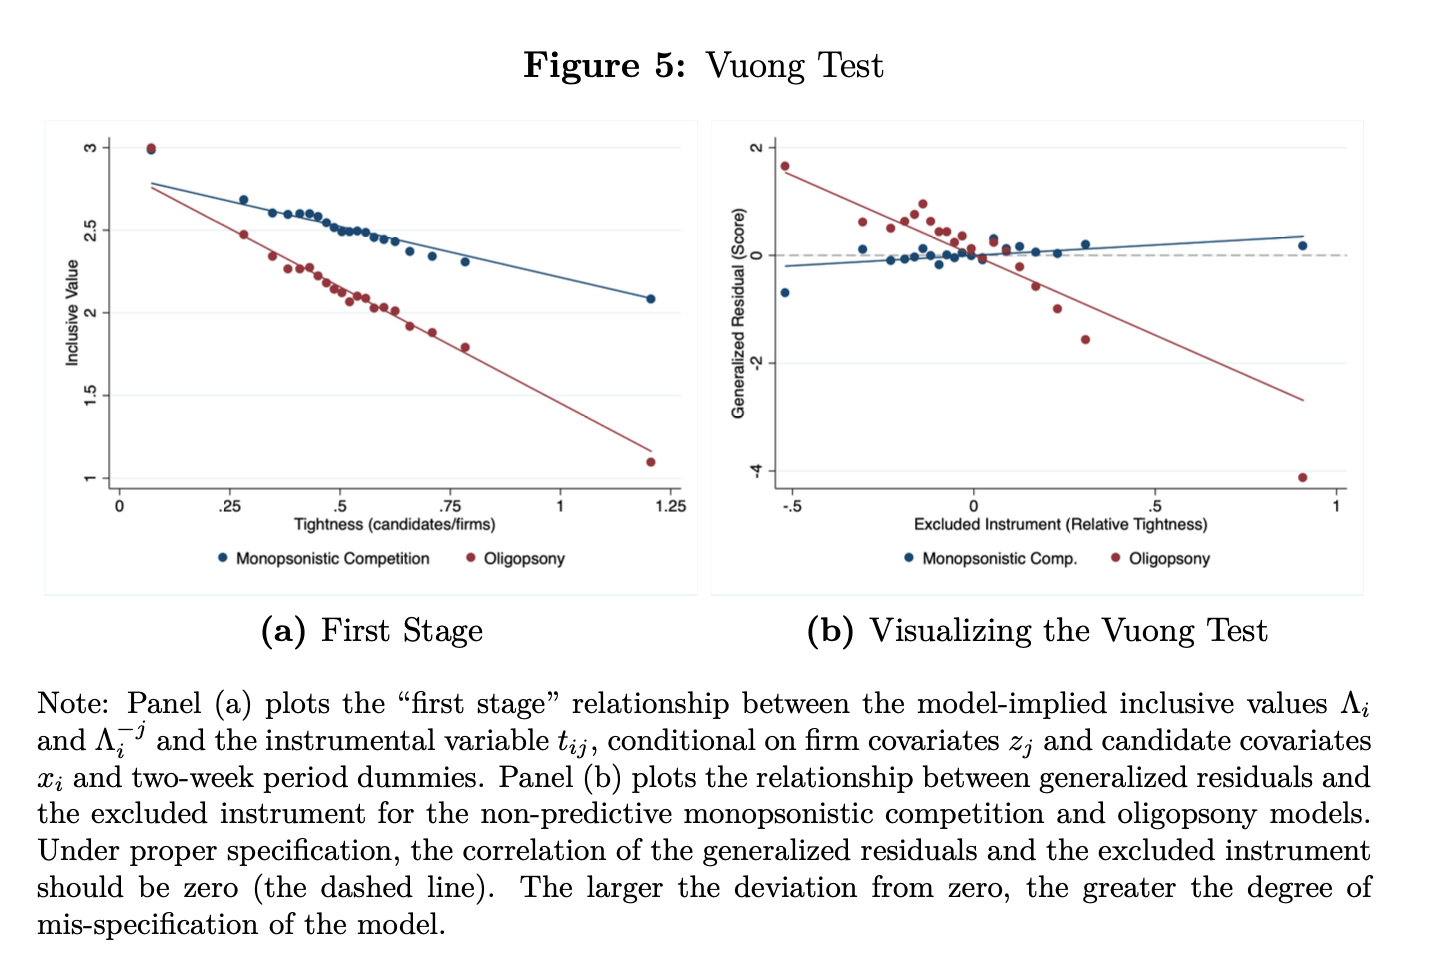
\includegraphics[height=0.9\textheight]{resources/scuderi1}
\end{column}
\begin{column}{0.3\textwidth}
\begin{itemize}
\item Offered wages for online job platform
\item Compares Monopsony vs. oligopolistic competition vs. perfect comp.
\item Compares tailored offers vs. not (price discrimination).
\end{itemize}
\end{column}
\end{columns}
\end{frame}


\begin{frame}{Scuderi JMP 2022: Models of Labor Supply}
\begin{columns}
\begin{column}{0.5\textwidth}
\begin{itemize}
\item Firms ignore competitors (Monopsony)
\item Firms offer wages independent of candidate characteristics (experience, demographics).
\item Firms are definitely NOT paying MPL.
\end{itemize}
\end{column}
\begin{column}{0.5\textwidth}
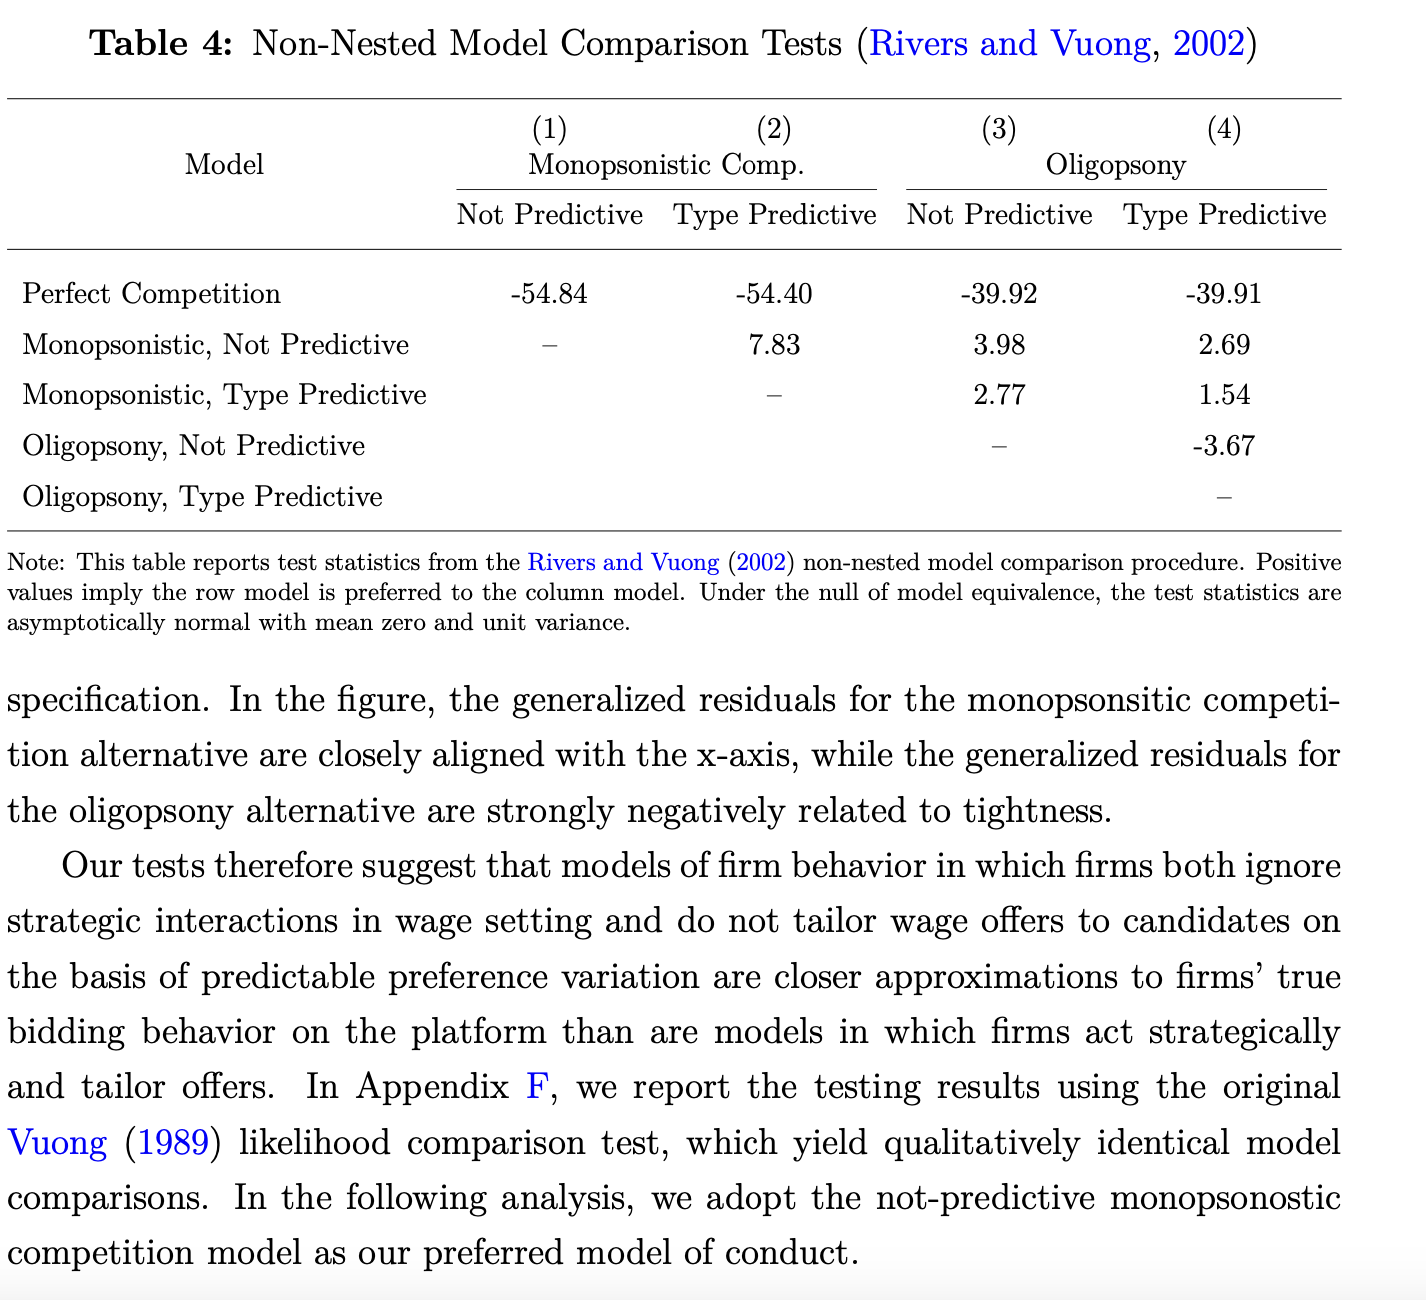
\includegraphics[height=0.9\textheight]{resources/scuderi2}
\end{column}
\end{columns}
\end{frame}


\begin{frame}{Starc Wollmann: Generic Pharma Cartel + Entry}
Do cartels encourage entry with high prices? Starc and Wollmann (2022) apply the BCS test to the generic-drug cartel; the menu is competitive vs.\ joint-profit-maximizing pricing before and after cartel formation, with non-members best responding.\\
\vspace{0.25cm}
\begin{quote}
in 2013, Teva Pharmaceuticals, the largest generic firm, hired NP, a marketing executive with especially strong industry relationships, and tasked her with "price increase implementation."1 Over an 18-month period, industry participants exchanged thousands of calls and texts—alongside countless LinkedIn, Facebook, and WhatsApp messages and face-to-face conversations—with contacts at rival firms to coordinate the increases (Complaint, page 322).2 Following this period, prescription drug expenditures by governments, private insurers, and individuals rose sharply by billions of dollars.
\end{quote}
\end{frame}


\begin{frame}{Starc Wollmann: Testing Results (prices rise with the cartel, less in markets that invite entry)}
\begin{center}
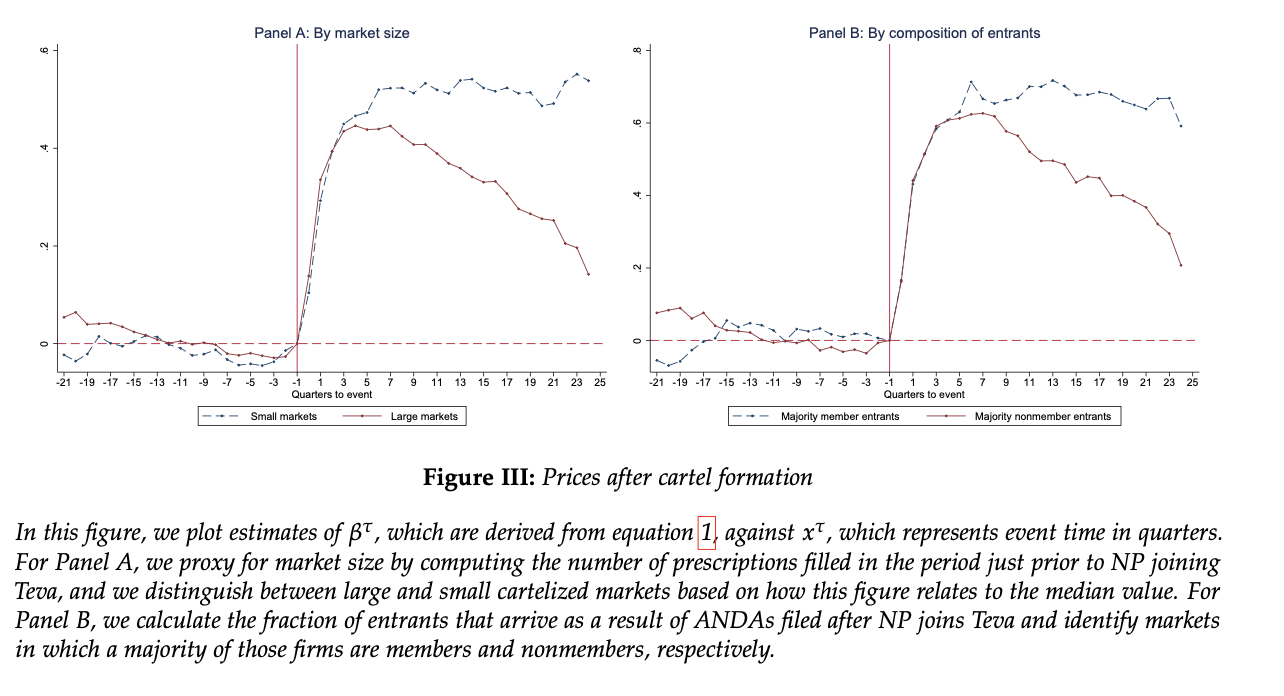
\includegraphics[height=0.85\textheight]{resources/starc_2}
\end{center}
\end{frame}


\section{Application: Common Ownership (Backus Conlon Sinkinson)}

\begin{frame}[plain]{What is the Common Ownership Hypothesis?}
\begin{itemize}
\item Economics starts from the premise that firms maximize profits.
\begin{itemize}
\item Friedman (1953): natural selection of firms and billiards players.
\item Or, firms answer to investors, \alert{maximize shareholder value}.
\item We generally think of these objectives as aligned (possibly subject to managers' agency frictions).
\end{itemize}
\item So what do investors want?
\begin{itemize}
\item Some (diversified) investors may hold stakes in you \textit{and your competitor}. These are called ``common owners.''
\item Common owners are harmed when managers engage in \alert{business stealing}.
\end{itemize}
\item As a theory of firm behavior in \alert{joint ventures} this is an old idea. The recent innovation is to extend this approach to \alert{passive or institutional investors}
\end{itemize}
\end{frame}


\begin{frame}[plain]{Rise of the Big Three (S\&P 500 components, BCS AEJ:Micro 2021)}
\begin{center}
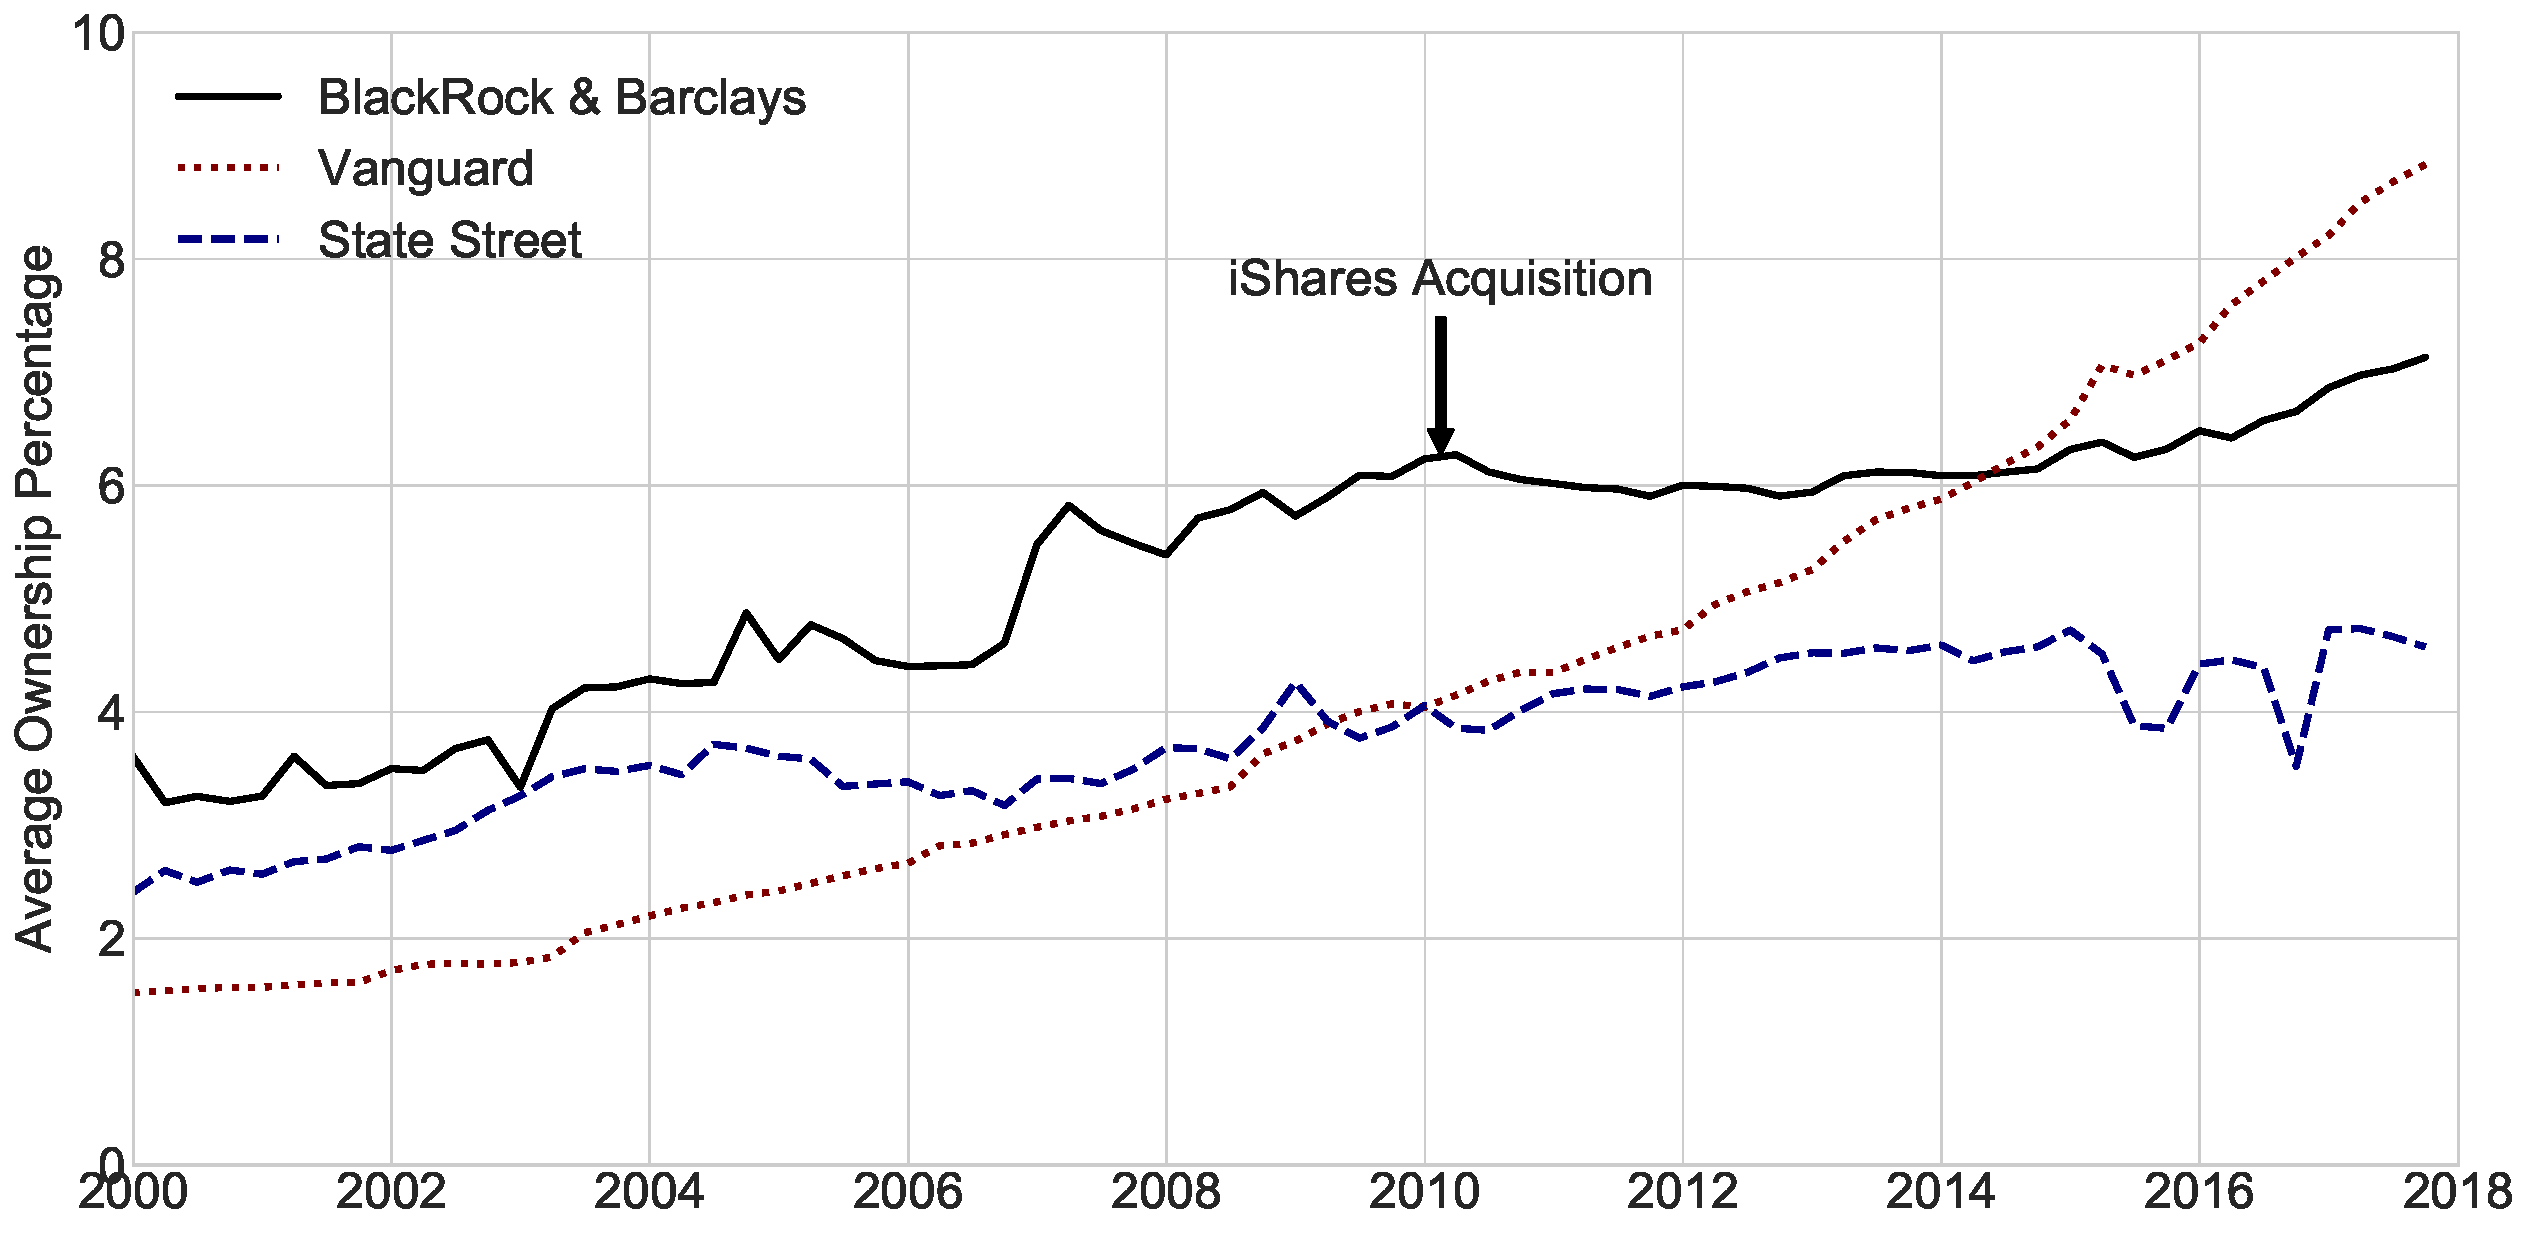
\includegraphics[height=0.9\textheight]{resources/figure5_big3.pdf}
\end{center}
\end{frame}


\begin{frame}{Some Reasonable (?) Assumptions (BCS 2020 P\&P)}
Most models of common ownership (implicitly) make the following assumptions:
\begin{description}
\item[Investor Portfolios] Investors are entitled to a share of profits $\beta_{fs}$ and hold portfolios $V_s = \sum_{f} \beta_{fs} \pi_f$
\item[Manager Agency (Rotemberg 1984)] Managers maximize a $(\gamma)$ weighted average of investor payoffs $Q_f = \sum_{s} \gamma_{fs} V_s$.
\end{description}
These are pretty general since $s$ could contain the manager herself.\\
\end{frame}


\begin{frame}{Derivation of Profit Weight}
\small
Easy to show:
\begin{align*}
Q_{f}\left(x_{f}, x_{-f}\right) &=\sum_{\forall s} \gamma_{f s} \cdot V_{s}\left(x_{f}, x_{-f}\right)\\
&\propto \pi_{f}+\sum_{g \neq f} \underbrace{\left(\frac{\sum_{\forall s} \gamma_{f s} \beta_{g s}}{\sum_{\forall s} \gamma_{f s} \beta_{f s}}\right)}_{\equiv \kappa_{f g}\left(\gamma_{f}, \beta\right)} \pi_{g}
\end{align*}
\begin{itemize}
    \item $\kappa_{fg}$ is interpreted as a \alert{profit weight}, where one dollar of profits at firm $g$ are valued as $\kappa_{fg}$ dollars in the objective function of firm $f$.
    \item Depends on two primitives: $\beta$ and $\gamma$.
\begin{itemize}
    \item $\beta$ (cash-flow rights) is often directly observable.
    \item $\gamma$ embeds a model of corporate governance. Literature assumes $\gamma = \beta$ (``proportional control").
\end{itemize}
\item Not specific to a particular strategic game: this is the $\mathcal{H}(\kappa)$ from our multiproduct Bertrand FOCs.
\end{itemize}
\end{frame}


\begin{frame}[plain]{The Reduced-Form Literature (and its Critics)}
\small
Symmetric homogeneous-good Cournot with profit weights gives a share-weighted average markup (with market demand elasticity $\epsilon$):
\begin{align*}
\sum_f s_f \cdot \frac{p - mc_f}{p} = \frac{1}{\epsilon} \underbrace{\symbf{s}' \, \mathcal{H}(\kappa) \, \symbf{s}}_{\equiv MHHI}, \qquad
MHHI\Delta \equiv MHHI - \underbrace{\symbf{s} \cdot \symbf{s}}_{HHI}
\end{align*}
Some regress
\begin{align*}
\log \left(p_{r j t}\right)=\beta_1 \cdot M H H I \Delta_{r t}+\beta_2 \cdot H H I_{r t}+\theta \cdot X_{r j t}+\alpha_t+\nu_{r j}+u_{r j t}
\end{align*}
\begin{itemize}
\item Azar, Schmalz, Tecu (JF 2018): airline routes with more common ownership have 3--7\% higher fares.
\item But $MHHI\Delta$ is a function of \alert{equilibrium market shares} -- endogenous! (O'Brien Waehrer 2017). Price-concentration regressions all over again.
\item Dennis, Gerardi, Schnitzler (JF 2022): not robust (driven by the share component); Kennedy, O'Brien, Song, Waehrer (2017): structural version finds nothing.
\item Better idea: treat CO vs.\ own-profit maximization as a \alert{conduct testing} problem.
\end{itemize}
\end{frame}


\begin{frame}{Cereal Data}
Main Dataset is NielsenIQ (from Kilts) from 2007-2017
\begin{itemize}
\item Consolidate to \texttt{dma-chain-week}.
\item Keep largest chains who price at chain level
\begin{itemize}
\item Select based on \# observations from panelist data.
\end{itemize}
\item Consolidate \texttt{upc} $\rightarrow$ \texttt{brand} (Honey Nut Cheerios) from multiple package sizes and box designs.
\begin{itemize}
\item Divide revenue by servings
\item Maintain the fiction that households purchase servings.
\end{itemize}
\end{itemize}
Why cereal? Long history as IO ``model organism'' (Nevo x 3), 4 big firms, and non-Nash behavior isn't so crazy (FTC case in the 1970s, 1990s cartel/price war).
\end{frame}


\begin{frame}[plain]{Cereal Data: Variation in $\kappa$}
\begin{center}
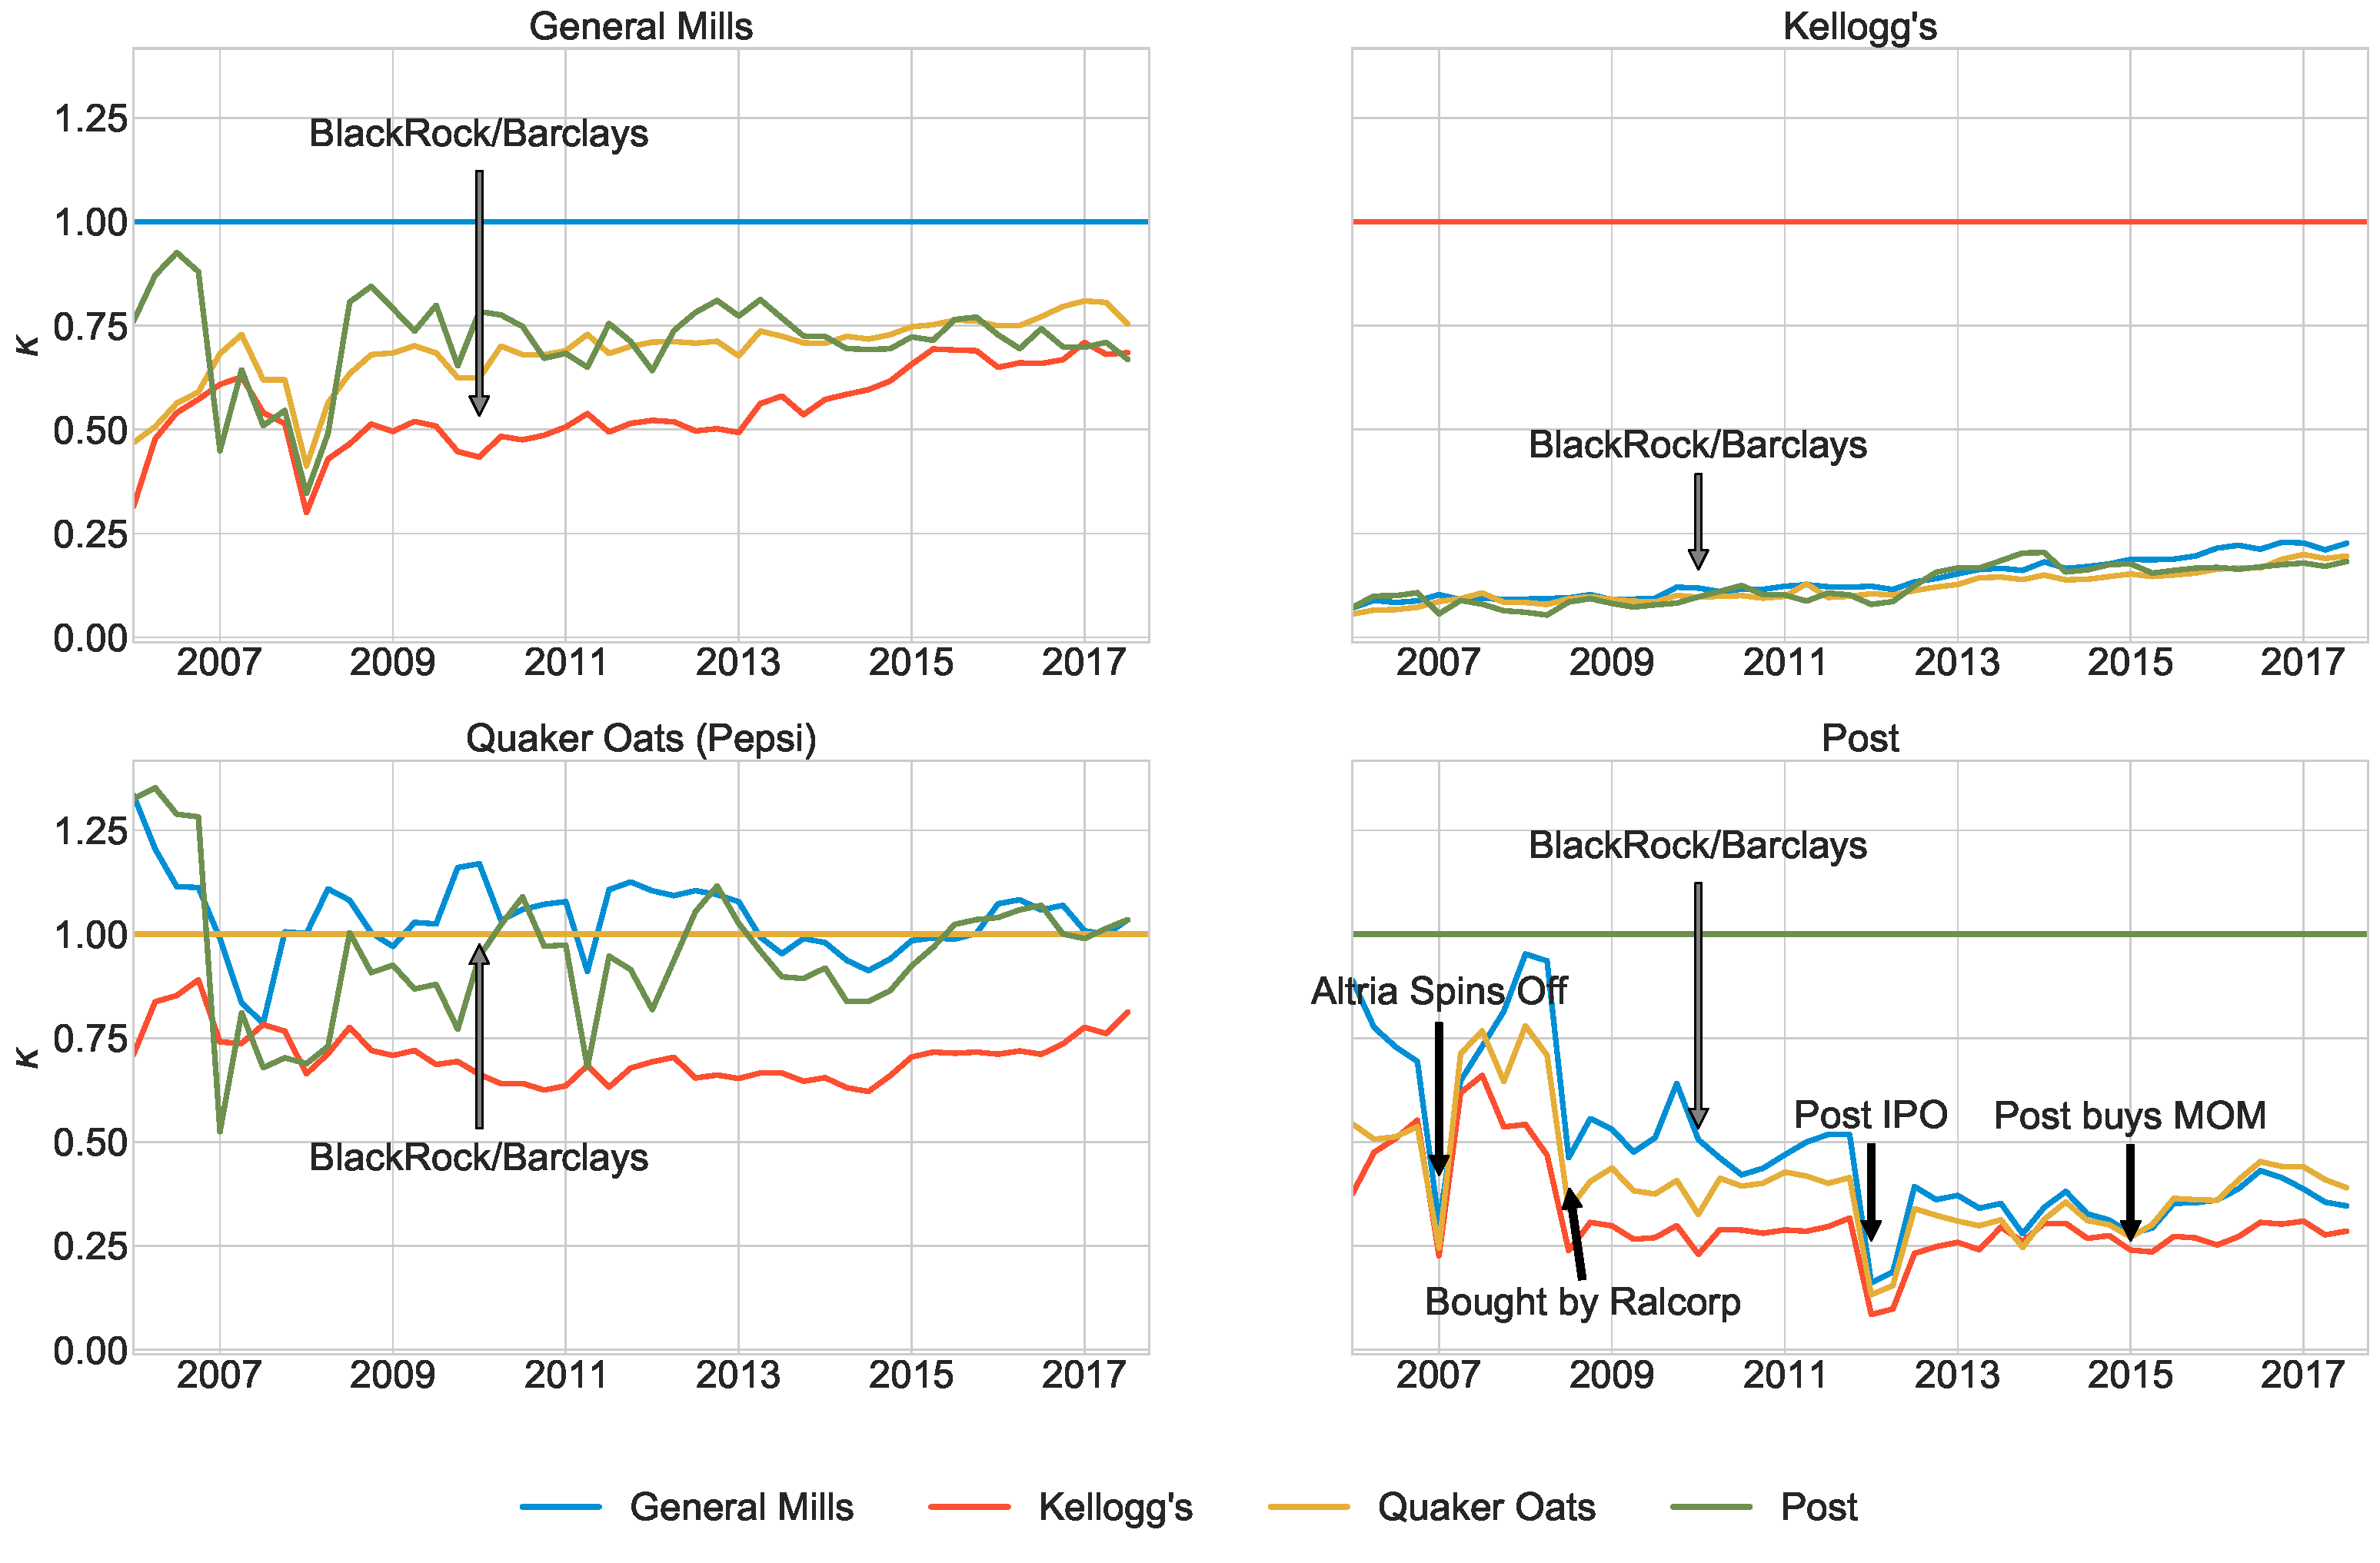
\includegraphics[height = 0.9\textheight ]{resources/cereal_kappas_alpha_1.pdf}
\end{center}
\end{frame}


\begin{frame}{Implementation: Demand Specification}
\begin{gather*}
u_{ijt} =  h_d(\textrm{x}_{jt}^{(1)}, \textrm{v}_{jt}; \theta_1) - \alpha\, p_{jt} + \lambda \, \log(\text{ad}_{jt})  + \left(\Sigma \, \nu_i + \Pi\, \textrm{y}_i \right) \cdot \textrm{x}_{jt}^{(2)}+ \xi_{jt} + \varepsilon_{ijt}\\
\end{gather*}
\vspace{-0.75cm}
\begin{itemize}
\item $\textrm{y}_i$ demographics: estimated at the $\texttt{dma-chain-year}$ level (from panelists); joint distribution of $(income, kids)$.
\item $\nu_i$ are random (normal) draws; price is lognormal.
\item Lots of FE in $h_d(\cdot)$ (product, chain-dma, year, week of year); estimated with \texttt{PyBLP} plus 520 micro-moments for $(\Pi,\Sigma)$.
\item Supply side/testing: exactly the machinery above -- compute $\eta_{jt}(\symbf{p},\symbf{s},\theta_2,\kappa)$ under each conduct model once, then rank by the scalar RV test and by the full conditional-moment norm.
\end{itemize}
\end{frame}


\begin{frame}{Possible Exclusion Restrictions}
We are looking for variables which affect \alert{demand but not supply}:
\begin{align*}
\sigma_{j}^{-1}(\symbf{s}_t, \symbf{p_t},\alert{\textrm{y}_t}, \textrm{x}_t,  \textrm{v}_t, \widetilde{\theta}_2)
&= h_d(\textrm{x}_{jt},\alert{ \textrm{v}_{jt}}; \theta_1) - \alpha\, p_{jt} + \lambda \, \log(\text{ad}_{jt})+ \xi_{jt} \\
p_{jt} - \eta_{jt}(\symbf{s}_t, \symbf{p_t}; \theta_2, \mathcal{H}_t(\kappa))
&= h_s(\textrm{x}_{jt}, \alert{\textrm{w}_{jt}}; \theta_3) + \omega_{jt}
\end{align*}
Things we use (ranked by strength for conduct, see the instrument table):
\begin{itemize}
    \item The demand-side optimal IV $\E[\partial\xi/\partial\theta \mid z]$ at a flexible $\widehat{\E}[p \mid z]$: strongest, conduct-agnostic.
    \item Demographics (enter nonlinearly): $\textrm{y}_t$ (chain-level income works well).
    \item Rivals' cost shifters $\textrm{w}_{-j,t}$ (the price of a grain the product does not use): valid, thin after FE.
    \item Characteristics of other goods $f(\textrm{x}_{-j,t})$ (BLP instruments): weakest for conduct.
    \item Obvious choice $\textrm{v}_{jt}$ (product recalls): too few events to matter.
\end{itemize}

Things we don't use:
\begin{itemize}
    \item Unobserved demand shocks $\xi_{jt}$ (see MacKay Miller 2020 for $Cov(\xi_j,\omega_j)=0$).
    \item Observable $\kappa$ conduct shifters (financial mergers/events, see Miller Weinberg (2018))
\end{itemize}
\end{frame}


\begin{frame}[plain,label=mainresults]{Published Results (BCS 2021, Table 8): Rivers--Vuong $\mathsf{T}$, $N(0,1)$}
\begin{center}
\scalebox{0.5}{\begin{tabularx}{500pt}{l*4             {>{\Centering}X}}\toprule
{} &  Others' Cost &  Demographics &  BLP Inst. &  Dmd. Opt. Inst. \\
\midrule \multicolumn{1}{c}{Own Profit Max vs.}&             \multicolumn{4}{c}{Panel 1: $A(\symbf{z}_t)=\symbf{z}_t,$ linear $h_s(\cdot)$ }\\                 \cmidrule(lr){1-1} \cmidrule(lr){2-5}
Single Product                            &        1.6489 &        1.1116 &     0.9977 &           1.6432 \\
Common Ownership                          &       -3.8928 &       -1.1957 &     0.5044 &          -1.0329 \\
Double Marginalization                    &        1.4435 &        0.9892 &    -0.0427 &           5.5684 \\
Common Ownership + Double Marginalization &       -0.1919 &        0.6815 &     0.1404 &           5.4688 \\
Perfect Competition                       &        1.1730 &        0.4171 &     0.7364 &           3.9589 \\
Monopolist                                &       -1.4097 &       -1.0680 &    -0.4523 &          -1.0908 \\

 \midrule 

\multicolumn{1}{c}{Own Profit Max vs.}& \multicolumn{4}{c}{Panel 2:             $A(\symbf{z}_t)=\mathbb{E}[\Delta \eta^{12}|\symbf{z_t}]$, linear $h_s(\cdot)$ and $g(\cdot)$}\\                            \cmidrule(lr){1-1} \cmidrule(lr){2-5}
Single Product                            &        1.4264 &        0.5795 &     0.6662 &           0.7516 \\
Common Ownership                          &       -2.3044 &       -0.5105 &    -0.0384 &          -1.4297 \\
Double Marginalization                    &        0.8644 &        0.4421 &    -0.5311 &           2.9800 \\
Common Ownership + Double Marginalization &       -0.9382 &       -0.2389 &    -0.3684 &           0.2460 \\
Perfect Competition                       &        0.7164 &        0.6135 &    -0.1080 &           1.8776 \\
Monopolist                                &       -0.8577 &       -0.4002 &    -0.3868 &          -1.1097 \\

 \midrule 

\multicolumn{1}{c}{Own Profit Max vs.}& \multicolumn{4}{c}{Panel 3:             $A(\symbf{z}_t)=\mathbb{E}[\Delta \eta^{12}|\symbf{z_t}]$, random forest $h_s(\cdot)$ and $g(\cdot)$}\\                    \cmidrule(lr){1-1} \cmidrule(lr){2-5}
Single Product                            &        5.0725 &        5.3347 &     5.2702 &           5.5758 \\
Common Ownership                          &       -3.9823 &       -3.6775 &    -4.0786 &          -4.3977 \\
Double Marginalization                    &       -6.3295 &       -9.9033 &    -6.5311 &          -7.6302 \\
Common Ownership + Double Marginalization &       -6.6568 &       -6.8735 &    -6.6624 &          -7.5578 \\
Perfect Competition                       &       -5.5005 &       -7.7749 &    -6.4083 &          -7.7653 \\
Monopolist                                &       -3.7240 &       -4.4602 &    -3.6134 &          -3.8959 \\
\bottomrule
\end{tabularx}
}
\end{center}
\end{frame}


\begin{frame}{Updated Results (BCS 2.0): Per-Model Criterion and Model Confidence Set}
\footnotesize
Full-CMR criterion $C \cdot \widehat{Q}(\eta^m)$ (smaller $=$ closer to $\E[\omega \mid z] = 0$) and the number of pairwise comparisons each model significantly loses (unified bootstrap); year$+$chain FE, boosting, controls partialled out of $z$, market clusters.
\begin{center}
\renewcommand{\arraystretch}{1.0}
\begin{tabular}{lrrr}
\toprule
model & \texttt{opt\_iv} $\;C\widehat{Q}$ (beaten) & \texttt{demog} (beaten) & \texttt{opc} (beaten) \\
\midrule
\textbf{single-product} & 34348 (\textbf{0}) & 87 (\textbf{0}) & 9.9 (0) \\
own-profit (Bertrand) & 35473 (1) & 106 (1) & 12.4 (0) \\
common ownership $\kappa$ & 35590--35790 (1--4) & 116--121 (1) & 8.3--14.5 (0) \\
monopoly (big 4) & 38261 (5) & 138 (\textbf{0}) & 12.7 (0) \\
monopoly (all) & 50763 (6) & 590 (6) & 449 (6) \\
\midrule
model confidence set & $\{$single$\}$ & $\{$single, monopoly-4$\}$ & all but monopoly-all \\
\bottomrule
\end{tabular}
\end{center}
\begin{itemize}
\item \textbf{Own-profit is the robust substantive winner}: it beats common ownership, monopoly, and perfect competition on every instrument with power. Same ordering as the published Table 8, and the scalar test agrees.
\item Only the optimal IV has the power to isolate a singleton set; the weaker groups rank the top of the ladder but cannot separate it.
\item Every $Q_m > 0$: this is ``rank the misspecified models,'' conditional on the demand-side instruments being excluded from the true cost shock.
\end{itemize}
\end{frame}


\begin{frame}{The Single-Product Puzzle}
\begin{itemize}
\item Single-product pricing (each brand ignores its sister brands) fits the moment condition \alert{better} than own-profit maximization. Robust across instruments, samples, fixed effects, weighting, learners, and both criteria; it is already in the 2021 Table 8 numbers.
\item It is \alert{not} ``no market power'': single-product markups are $1/(\alpha(1-\sigma_j))$-sized, comfortably above cost. It says firms appear to internalize \alert{less} cross-brand recapture than Bertrand with the estimated demand implies.
\item Candidate explanations, none settled:
\begin{enumerate}
\item Demand misspecification: the cross-price elasticities (recapture) are mismeasured, so the ``correct'' internalization looks wrong through the lens of this demand system. Recall the micro-data week: substitution patterns are the thing BLP gets least right.
\item Rule-of-thumb pricing: brand managers price their own brand; the corporate parent does not reprice Cheerios when Lucky Charms moves.
\item Another instrument or moment may reorder single vs.\ own-profit; nothing we have tried does.
\end{enumerate}
\item Methodological point: a result like this only becomes visible once the test is honest about ranking misspecified models. A specification test would have rejected everything and said nothing.
\end{itemize}
\end{frame}


\begin{frame}[plain]{An Internalization Parameter}
Let $\kappa$ represent the weight a firm places on competitors and $\tau$ the internalization of those weights.
 \begin{equation*}
 arg\max_{p_j \,:\, j \in \calJ_f} \sum_{j \in \calJ_f} (p_j - mc_j) \cdot \sigma_j(\symbf{p})+
 \sum_{g\neq f} \alert{\tau} \kappa_{fg} \sum_{j \in \calJ_g} (p_k - mc_k) \cdot \sigma_k(\symbf{p})
 \end{equation*}
Now,
\begin{itemize}
\item $\tau = 0$ implies own-profit maximization
\item $\tau = 1$ implies common ownership pricing
\item $\tau$ in between is..? Agency?
\end{itemize}
We test $\tau \in (0.1, \ldots, 0.9)$ against own-profit maximization.
\end{frame}


\begin{frame}[plain]{Internalization Parameter Results}
\begin{center}
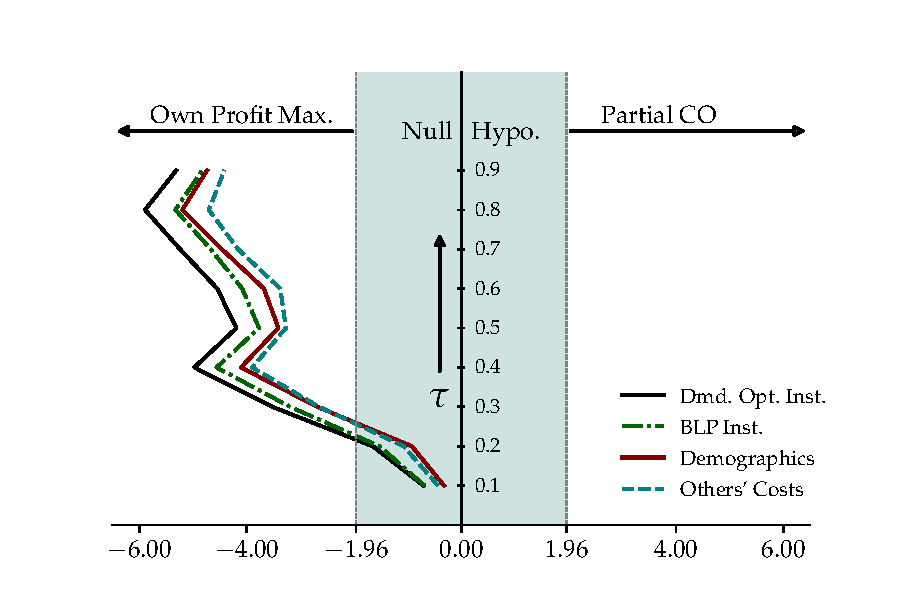
\includegraphics[width=10cm]{resources/tau_figure2.pdf}
\end{center}
\end{frame}


\begin{frame}[plain]{Stepping Back: What About the Mechanism?}
\begin{itemize}
\item In RTE cereal, we see strong evidence in favor of own-profit maximization rather than common ownership pricing, on the published test and on BCS 2.0 alike.
\item In some sense this is a \alert{frictionless} model
\begin{itemize}
  \item Managers do exactly what investment managers want
  \item Investment managers seek to maximize \alert{portfolio value}
\end{itemize}
\item Some attempts at micro foundations are questionable
\begin{itemize}
  \item Anton, Ederer, Gine, Schmalz: toy model has manager choose effort to reduce $mc$.
  \item Weaker managerial incentives: higher $mc$ and higher $p$
  \item Some correlation that executives at commonly owned firms have performance less correlated with profitability.
\end{itemize}
\item In some sense CO is what we would see absent agency problems, so where are they?
\end{itemize}
\end{frame}


\section{Thanks!}

\end{document}
